\documentclass{sigplanconf}
\usepackage[utf8]{inputenc}
\usepackage{epsfig}
\usepackage{multicol}
\usepackage{multirow}
\usepackage{wrapfig}
\usepackage{subfigure}
\usepackage{fancyvrb}
\usepackage{url}
\usepackage{balance}
\usepackage{listings}
\usepackage{multicol}
\lstset{language=C, basicstyle=\ttfamily, breaklines=true, frame=lines}
\makeatletter{}\usepackage{latexsym}
\usepackage{amssymb}            \usepackage{stmaryrd}           
\newcommand{\m}[1]{\mathsf{#1}}
\newcommand{\f}[1]{\framebox{#1}}

\newcommand{\eph}{\mathit{eph}}
\newcommand{\pers}{\mathit{pers}}
\newcommand{\um}[1]{\underline{\m{#1}}}

\newcommand{\seq}{\vdash}
\newcommand{\semi}{\mathrel{;}}
\newcommand{\lequiv}{\mathrel{\dashv\vdash}}

\newcommand{\lolli}{\multimap}
\newcommand{\tensor}{\otimes}
\newcommand{\with}{\mathbin{\binampersand}}
\newcommand{\paar}{\mathbin{\bindnasrepma}}
\newcommand{\one}{\mathbf{1}}
\newcommand{\zero}{\mathbf{0}}
\newcommand{\bang}{{!}}
\newcommand{\whynot}{{?}}
\newcommand{\bilolli}{\mathrel{\raisebox{1pt}{\ensuremath{\scriptstyle\circ}}{\lolli}}}

 


\begin{document}

\special{papersize=8.5in,11in}
\setlength{\pdfpageheight}{\paperheight}
\setlength{\pdfpagewidth}{\paperwidth}
\conferenceinfo{PPDP '14}{September 8--10, 2014, Canterbury, UK}
\copyrightyear{2014}
\copyrightdata{978-1-4503-2947-7/14/09}
\doi{2643135.2643150}

\exclusivelicense                                                                                                                      

\title{Design and Implementation of a Multithreaded Virtual Machine for Executing Linear Logic Programs}

\authorinfo{Flavio Cruz}
           {Carnegie Mellon University\\Pittsburgh, PA 15213, USA}
           {fmfernan@cs.cmu.edu}

\authorinfo{Ricardo Rocha}
           {CRACS \& INESC TEC\\University of Porto\\Rua Campo Alegre 1021/1055\\4169-007 Porto, Portugal}
           {ricroc@dcc.fc.up.pt}

\authorinfo{Seth Copen Goldstein}
           {Carnegie Mellon University\\Pittsburgh, PA 15213, USA}
           {seth@cs.cmu.edu}


\maketitle

\makeatletter{}\begin{abstract}
Linear Meld is a concurrent forward-chaining linear logic programming
language where logical facts can be asserted and retracted in a
structured way. In Linear Meld, a program is seen as a database of
logical facts and a set of derivation rules. The database of facts is
partitioned by the nodes of a graph structure which leads to
parallelism when nodes are executed simultaneously. Due to the
foundations on linear logic, rules can retract facts in a declarative
and structured fashion, leading to more expressive programs. We
present the design and implementation of the virtual machine that we
implemented to run Linear Meld on multicores, with particular focus on
thread management, code organization, fact indexing, rule execution,
and database organization for efficient fact insertion, lookup and
deletion. Our results show that the virtual machine is
capable of scaling programs with up to 16 threads and also exhibits
interesting scalar performance results due to our indexing optimizations.
\end{abstract}

\category{D.1.3}{PROGRAMMING TECHNIQUES}{Concurrent Programming}[Parallel Programming]
\category{D.3.4}{PROCESSORS}{Interpreters}
\category{D.3.4}{PROCESSORS}{Run-time environments}

\terms{Design, Languages, Performance}

\keywords{Linear Logic, Virtual Machine, Implementation}
 
\makeatletter{}\section{Introduction}

The last decade has seen a tremendous growth in content available in
the World Wide Web, and, more specifically, in information generated
from online social networks. The structure of such content is usually
a graph, a very flexible structure suited to represent content where
pairs of items are linked.  In order to process such information,
there has been an increased interest in running graph-based algorithms
concurrently and efficiently on top of distributed networks and
computer architectures (multicores).  Currently available libraries
and frameworks are built on top of imperative programming languages,
which require the programmer to know how to properly use the framework
and the language. Reasoning about such programs requires knowing the
intricacies of the framework, how computation is scheduled and how
processing units coordinate between each other.

Some well known frameworks include Dryad, Pregel and GraphLab.  The
Dryad system~\cite{Isard:2007:DDD:1272996.1273005} combines
computational vertices with communication channels (edges) to form a
data-flow graph. The program is scheduled to run on multiple
processors or cores and data is partitioned during runtime. Routines
that run on computational vertices are sequential, with no
synchronization.  The Pregel
system~\cite{Malewicz:2010:PSL:1807167.1807184} is also graph based,
although programs have a more strict structure. They must be
represented as a sequence of iterations where each iteration is
composed of computation and message passing.  Pregel is specially
suited to work on big graphs and to scale to large architectures.
GraphLab~\cite{GraphLab2010} is a C++ framework for developing
parallel machine learning algorithms. While Pregel uses message
passing, GraphLab allows nodes to have read/write access to different
scopes through different concurrent access models in order to balance
performance and data consistency. While some programs only need to
access the local node's data, others may need to update edge
information. Each consistency model will provide different guarantees
that are better adapted to some algorithms. GraphLab also provides
different schedulers that dictate the order in which node's are
computed.

Logic programming is an attractive approach to the graph-based algorithms,
since logic-based languages provide a high-level, declarative approach
to programming. An important characteristic of logic programming is
that it offers great potential for implicit parallelism, thus making
logic programs much easier to parallelize than imperative
programs. First, logic programs are easier to reason about since they
are based on logical foundations. Second, logic programmers do not
need to use low level programming constructs such as locks or
semaphores to coordinate parallel execution, because logic systems
hide such details from the programmer.

Logic programming split into two main groups:
\emph{backwards-chaining} and \emph{forward-chaining} languages. In a
backwards-chaining programming language, programs are composed of a
set of rules that can be activated by inputting a query. Given a query
$q(\hat{x})$, an interpreter will work backwards by matching
$q(\hat{x})$ against the head of a rule. If found, the interpreter
will then try to match the body of the rule, recursively, until it
finds the program axioms (rules without body). If the search procedure
succeeds, the interpreter finds a valid substitution for the $\hat{x}$
variables. A popular backwards-chaining programming language is
Prolog~\cite{Colmerauer:1993:BP:154766.155362}, which has been a
productive research language for executing logic programs in
parallel. Researchers took advantage of Prolog's non-determinism to
evaluate subgoals in parallel with models such as
\emph{And-parallelism} and
\emph{Or-parallelism}~\cite{Gupta:2001:PEP:504083.504085}.

In a forward-chaining logic programming language, programs start with
a database of facts (filled with the program's axioms) and a set of
logical rules. The database of facts is then used to fire the
program's rules and derive new facts that are then added to the
database. This process is repeated recursively until the database
reaches \emph{quiescence} and no more information can be derived from
the program. A popular forward-chaining programming language is
Datalog~\cite{Ramakrishnan93asurvey}.

We have designed Linear Meld~(LM), a forward-chaining logic programming
language that is specially suited for
concurrent programming over graph structures~\cite{cruz-iclp14}. LM
differs from Datalog-like languages because it integrates both
classical logic and linear logic~\cite{girard-87} into the language, allowing some
facts to be retracted and asserted in a logical fashion. Although most
Datalog and Prolog-like programming languages allow some kind of state
manipulation~\cite{Liu98extendingdatalog}, those features are
extra-logical, reducing the advantages brought forward by logic programming.

The roots of LM are the P2 system~\cite{Loo-condie-garofalakis-p2} and
the original Meld
language~\cite{ashley-rollman-derosa-iros07wksp,ashley-rollman-iclp09}. P2
is a Datalog-like language that maps a computer network to a graph,
where each computer node can perform computations locally and
communicate with neighbors. Meld is inspired by the P2 system
but adapted to the concept of massively distributed systems made of
modular robots with a dynamic topology. LM still follows the same
graph model of computation of Meld, which makes LM programs naturally
concurrent since the graph of nodes can be easily partitioned to be
executed by different threads. As a forward-chaining linear logic
programming language, LM also shares similarities with Constraint
Handling Rules
(CHR)~\cite{Betz:2005kx,DBLP:journals/corr/abs-1006-3039}.  CHR is a
concurrent committed-choice constraint language used to write
constraint solvers. A CHR program is a set of rules and a set of
constraints (which can be seen as facts). Constraints can be consumed
or generated during the application of rules. Some optimizations
used in LM such as join optimizations and the use of different data
structures for indexing facts were inspired by research done in
CHR~\cite{DBLP:journals/corr/cs-PL-0408025}.

In this paper, we present the design and implementation of the LM virtual machine
and compiler.
The LM virtual machine was designed from scratch to run LM programs on
multicore machines in an efficient manner\footnote{Source code available at \url{http://github.com/flavioc/meld}}.
The virtual machine is multithreaded and executes byte-code that is generated
by the LM compiler. To test our language and virtual machine we have implemented several graph algorithms, search
algorithms and machine learning algorithms, including: belief
propagation~\cite{Gonzalez+al:aistats09paraml}, belief propagation
with residual splash~\cite{Gonzalez+al:aistats09paraml}, PageRank,
graph coloring, N-Queens, shortest path, diameter estimation, map
reduce, quick-sort, neural network training, minimax, etc.

Our results show that our virtual machine is scalable and presents some interesting
execution times when compared with other competing systems.
The virtual machine uses a simple, but effective, work stealing algorithm
that is able to balance the load across threads, improving scalability.
Another important feature of our virtual machine is the dynamic indexing algorithm.
It is a runtime algorithm that decides how to index logical facts and which
data structure is best to use, so that database lookup and insertion time during rule application
is effectively reduced.

This remainder of the paper is organized as follows. First, we briefly
introduce the LM language. Then, we present an overview of the virtual
machine and describe in more detail the code organization, thread
management, rule execution and database organization. Finally, we
present our experiments and outline some conclusions.
 
\makeatletter{}\newcommand{\selector}[0]{[~S~\Rightarrow~y;~BE~] \lolli HE}
\newcommand{\comprehension}[0]{\{~\widehat{x};~BE;~SH~\}}
\newcommand{\aggregate}[0]{[~A~\Rightarrow~y;~\widehat{x};~BE;~SH_1;~SH_2~]}


\section{The LM Language}
\label{lm_language}

Linear Meld (LM) is a logic programming language that offers a
declarative and structured way to manage mutable state.  A program consists of
a database of facts and a set of derivation rules. The database
includes persistent and linear facts. Persistent facts cannot be
deleted, while linear facts can be asserted and retracted.

The dynamic (or operational) semantics of LM is identical to
Datalog. Initially, we populate the database with the \emph{program's axioms} (initial facts)
and then determine which derivation rules can be applied by
using the current database. Once a rule is applied, new facts can be
derive, which are then added to the database. If a rule uses linear
facts, they are retracted from the database. The program stops when
\emph{quiescence} is achieved, i.e., when rules no longer apply.

Each fact is a predicate on a tuple of \emph{values}, where the type
of the predicate prescribes the types of the arguments.  LM rules are
type-checked using the predicate declarations in the header of the
program. LM has a simple type system that includes types such as
\emph{node}, \emph{int}, \emph{float}, \emph{string},
\emph{bool}. Recursive types such as \emph{list X} and \emph{pair X;
  Y} are also allowed.  Each rule in LM has a defined priority that is
inferred from its position in the source file.  Rules at the beginning
of the file have higher priority.
We consider all the new facts that have been not used yet to create a
set of \emph{candidate rules}.
The set of candidate rules is then applied (by priority)
and updated as new facts are derived.


\subsection{Example}

\begin{figure}[ht]
{\footnotesize
\begin{Verbatim}[numbers=right]
type left(node, node).
type right(node, node).
type linear value(node, int, string).
type linear replace(node, int, string).

// set of rules
replace(A, K, New),
value(A, K, Old)
   -o value(A, K, New). // we found our key

replace(A, RKey, RValue),
value(A, Key, Value),
!left(A, B),
RKey < Key
   -o value(A, Key, Value),
      replace(B, RKey, RValue). // go left

replace(A, RKey, RValue),
value(A, Key, Value),
!right(A, B),
RKey > Key
   -o value(A, Key, Value),
      replace(B, RKey, RValue). // go right

// initial configuration
!left(@0, @1).     !right(@0, @2).
!left(@1, @3).     !right(@1, @4). 
!left(@2, @5).     !right(@2, @6).

value(@0, 3, a).   value(@1, 1, b).
value(@2, 5, c).   value(@3, 0, d).
value(@4, 2, e).   value(@5, 4, f).
value(@6, 6, g).

// update key 6 to value x
replace(@0, 6, x).
\end{Verbatim}
}
\caption{LM program for replacing a key's value in a binary tree dictionary}
\label{code:btree_replace}
\end{figure}

We now present in Fig.~\ref{code:btree_replace}, a LM program that
implements the update operation for a binary tree dictionary
represented as key/value pairs. We first declare the predicates (lines
1-4) which represent the facts we are going to use. Predicate
\texttt{left/2} and \texttt{right/2} are persistent while predicates
\texttt{value/3} and \texttt{replace/3} are linear. Predicate
\texttt{value/3} assigns a key/value pair to a tree node and predicate
\texttt{replace/3} represents an update operation that updates the key
in the second argument to the value in the third argument.

The algorithm uses three rules for the three cases of updating a key's
value: the first rule performs the update (lines 6-9); the second rule
recursively picks the left branch for the update operation (lines
11-16); and the third rule picks the right branch (lines 18-23). The
initial axioms are presented in lines 26-33 and they describe the
initial binary tree configuration, including keys and values.
Finally, with the \texttt{replace(@0, 6, x)} axiom instantiated at the
root node \texttt{@0} (line 36), we intend to change the value of key
6 to value \texttt{x}. Note that when writing rules or axioms,
persistent facts are preceded with a `\texttt{!}'.

Figure~\ref{fig:btree_trace} illustrates the trace of the
execution. Note that the program database is partitioned by the tree
nodes using the first argument of each fact. In
Fig.~\ref{fig:btree_trace1}, we present the database filled with the
program's axioms. Next, we follow the right branch using rule 3 since
$6 > 3$ (Fig.~\ref{fig:btree_trace2}). We then use the same rule
again in Fig.~\ref{fig:btree_trace3} where we finally reach the key
6. Here, we apply rule 1 and \texttt{value(@6, 6, g)} is updated to
\texttt{value(@6, 6, x)} (Fig.~\ref{fig:btree_trace4}).

\begin{figure*}[t]
\centering
\subfigure[Initial database]
   {\label{fig:btree_trace1}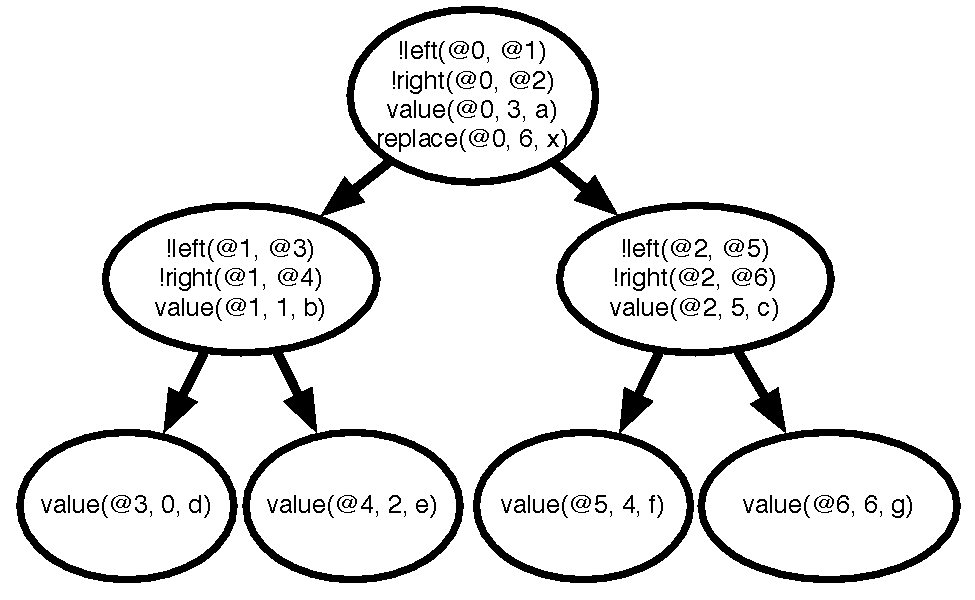
\includegraphics[width=0.44\textwidth]{figures/btree_trace1.pdf}}
\subfigure[After applying rule 3 at node $@0$]
   {\label{fig:btree_trace2}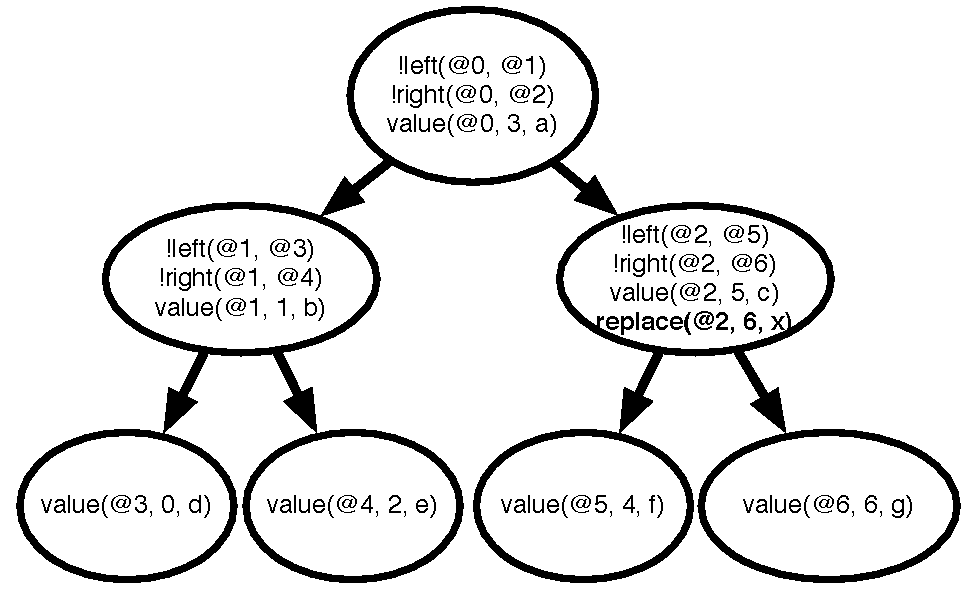
\includegraphics[width=0.44\textwidth]{figures/btree_trace2.pdf}}
\subfigure[After applying rule 3 at node $@2$]
   {\label{fig:btree_trace3}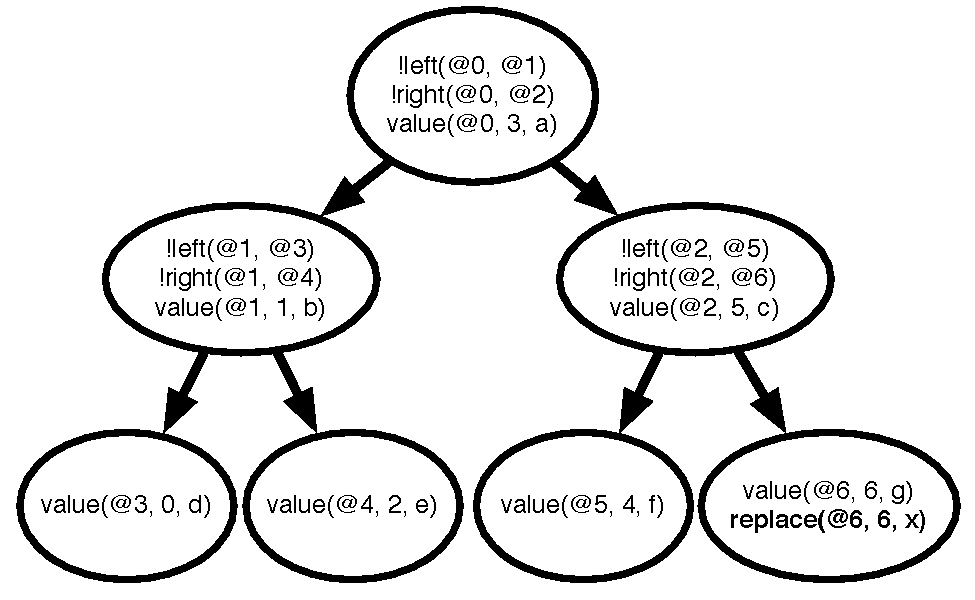
\includegraphics[width=0.44\textwidth]{figures/btree_trace3.pdf}}
\subfigure[After applying rule 1 at node $@6$]
   {\label{fig:btree_trace4}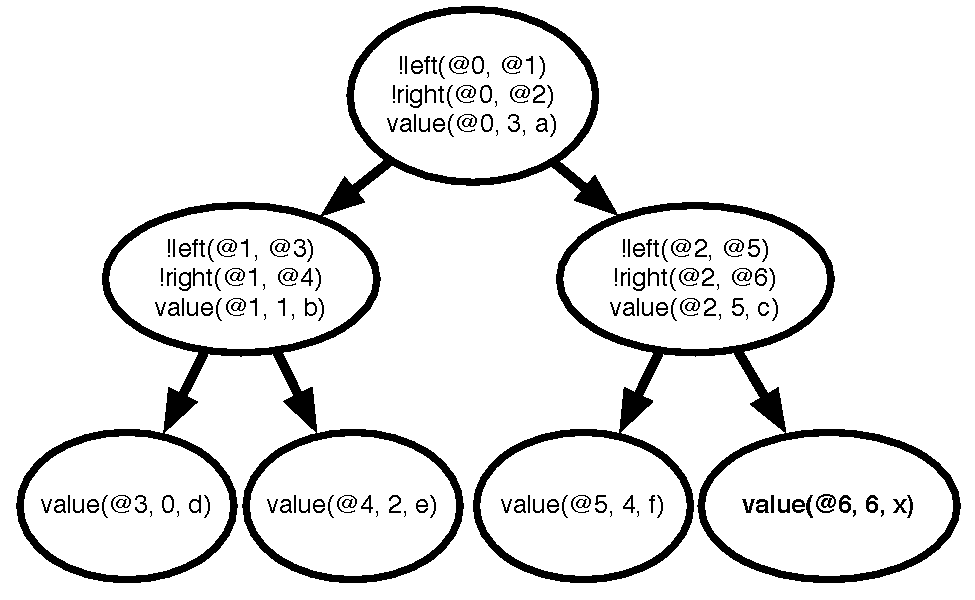
\includegraphics[width=0.44\textwidth]{figures/btree_trace4.pdf}}
\caption{An execution trace for the binary tree dictionary program}
\label{fig:btree_trace}
\end{figure*}


\subsection{Syntax}

Table~\ref{tbl:ast} shows the abstract syntax for rules in LM.  An LM
program $Prog$ consists of a set of derivation rules $\Sigma$ and a
database $D$.  Each derivation rule $R$ can be written as $BE \lolli
HE$ where $BE$ is the body of a rule and $HE$ is the head. Rules
without bodies are allowed in LM and they are called
\textit{axioms}. Rules without heads are also allowed.  The body of a
rule, $BE$, may contain linear ($L$) and persistent ($P$) \emph{fact
  expressions} and constraints ($C$). Fact expressions are template
facts that instantiate variables (from facts in the
database). Variables can be used again in the body for matching and
also in the head when instantiating facts. Constraints are boolean
expressions that must be true in order for the rule to be
fired. Constraints use variables from fact expressions and are built
using a small functional language that includes mathematical
operations, boolean operations, external functions and literal values.
The head of a rule, $HE$, contains linear ($L$) and persistent ($P$)
\emph{fact templates} which are uninstantiated facts to derive new
facts. Head expressions may use the variables instantiated in the
body. The head can also have \emph{comprehensions} ($CE$) and
\emph{aggregates} ($AE$).

\begin{table}[ht]
\centering
{\scriptsize
\begin{tabular}{llcl}
Program          & $Prog$ & $::=$ & $\Sigma, D$ \\
Set of Rules     & $\Sigma$ & $::=$ & $\cdot \; | \; \Sigma, R$\\
Database         & $D$ & $::=$ & $\Gamma; \Delta$ \\
Rule             & $R$ & $::=$ & $BE \lolli HE \; | \; \forall_{x}. R$ \\
Body Expression  & $BE$ & $::=$ & $L \; | \; P \; | \; C \; | \; BE, BE \; | \; \exists_{x}. BE \; | \; 1$\\
Head Expression  & $HE$ & $::=$ & $L \; | \; P \; | \; HE, HE \; | \; CE \; | \; AE \; | \; 1$\\
Linear Fact      & $L$ & $::=$ & $l(\hat{x})$\\
Persistent Fact  & $P$ & $::=$ & $\bang p(\hat{x})$\\
Constraint       & $C$ & $::=$ & $c(\hat{x})$ \\
Comprehension    & $CE$ & $::=$ & $\comprehension$ \\
Aggregate        & $AE$ & $::=$ & $\aggregate$ \\
Operations       & $A$ & $::=$ & $\mathtt{min} \; | \; \mathtt{max} \; | \; \mathtt{sum} \; | \; \mathtt{count}$ \\
Sub-Head         & $SH$ & $::=$ & $L \; | \; P \; | \; SH, SH \; | \; 1$\\
Linear Facts     & $\Delta$ & $::=$ & $\cdot \; | \; \Delta, l(\hat{t})$ \\
Persistent Facts & $\Gamma$ & $::=$ & $\cdot \; | \; \Gamma, \bang p(\hat{t})$ \\
\end{tabular}
}
\caption{Abstract syntax of LM}
\label{tbl:ast}
\end{table}

We created the concept of comprehensions to be used when the
consumption of a linear fact should generate a set of facts
accordingly to the current contents of the database. In a
comprehension $\comprehension$, $\widehat{x}$ is a list of variables,
$BE$ is the body of the comprehension and $SH$ is the head. The body
$BE$ is used to generate all possible combinations for the head $SH$,
according to the facts in the database. The following program shows a
simple example that uses comprehensions:

{\footnotesize
\begin{Verbatim}
!edge(@1, @2).
!edge(@1, @3).
iterate(@1).

iterate(A)
   -o {B | !edge(A, B) | perform(B)}.
\end{Verbatim}
}

When the rule is fired, we consume \texttt{iterate(@1)} and then
generate the comprehension. Here, we iterate through all the
\texttt{edge/2} facts that match \texttt{!edge(@1, B)}, which are
\texttt{!edge(@1, @2)} and \texttt{!edge(@1, @3)}. For each fact, we
then derive \texttt{perform(B)}, namely \texttt{perform(@2)} and
\texttt{perform(@3)} in this example.

Another useful feature is the ability to reduce several facts into a
single fact. For that, we have aggregates, a special kind of sub-rule
that works very similarly to comprehensions. In a aggregate
$\aggregate$, $A$ is the aggregate operation, $\widehat{x}$ is the
list of variables introduced in $BE$, $SH_1$ and $SH_2$ and $y$ is the
variable in the body $BE$ that represents the values to be aggregated
using $A$. Like comprehensions, we use $\widehat{x}$ to try all the
combinations of $BE$, but, in addition to deriving $SH_1$ for each
combination, we aggregate the values represented by $y$ and derive
$SH_2$ only once using $y$. As an example, consider the following
program:

{\footnotesize
\begin{Verbatim}
price(@1, 3).
price(@1, 4).
price(@1, 5).
count-prices(@1).

count-prices(A)
   -o [sum => P | . | price(A, P) | 1 | total(A, P)].
\end{Verbatim}
}

By applying the rule, we consume \texttt{count-prices(@1)} and derive
the aggregate which consumes all the \texttt{price(@1, P)} linear
facts. These are summed up and \texttt{total(@1,~12)} is derived. LM
provides several aggregate operations, including the \emph{minimum},
\emph{maximum}, \emph{sum} and \emph{count}. Note that the \texttt{.} syntax indicates
an empty list of variables and \texttt{1} is borrowed from linear logic
and represents an empty derivation.

Comprehensions and aggregates are logically justified by the underlying
proof system of the language. Our proof system is extended with greatest
fixed points~\cite{Baelde:2012:LGF:2071368.2071370}, which allows us to describe
recursive definitions such as comprehensions or aggregates.
A more detailed description is found in~\cite{cruz-iclp14}.


\subsection{Concurrency}

LM is at its core a concurrent programming language. The database of
facts can be seen as a graph data structure where each node contains a
fraction of the database.  To accomplish this, we force the first
argument of each predicate to be typed as a \emph{node}. We then
restrict the derivation rules to only manipulate facts belonging to a
single node.  However, the expressions in the head may refer to other
nodes, as long as those nodes are instantiated in the body of the
rule.

Due to the restrictions on LM rules, nodes are able to run rules
independently without using other node's facts. Node computation
follows a \emph{don't care} or \emph{committed choice} non-determinism
since any node can be picked to run as long as it contains enough
facts to fire a derivation rule.  Facts coming from other nodes will
arrive in order of derivation but may be considered partially and
there is no particular order among the neighborhood. To improve
concurrency, the programmer is encouraged to write rules that take
advantage of the non-deterministic nature of execution since too much
determinism will naturally imply less scalability and more synchronization
when executing the programs.
 
\makeatletter{}\section{The Virtual Machine}
\label{virtual_machine}

We have developed a compiler that compiles LM programs to byte-code
and a multithreaded virtual machine (VM) using POSIX threads
that runs the byte-code.


\subsection{Threads}

A key goal of our design is to keep the threads as busy as possible
and to reduce inter-thread communication. When the VM starts, it reads
the byte-code file and starts all threads. Initially, the VM will
partition the application graph of $N$ nodes into $T$ subgraphs (the
number of threads) and then each thread will work on their own
subgraph. Reduction of communication between nodes in different threads
is achieved by first ordering the node addresses present in the code in such a way that
connected nodes are clustered together and then partitioning them to
threads. During compilation, we take note of predicates that are used
for communication (arguments with type \emph{node}) and
then build a graph of nodes from them. The nodes of
the graph are then ordered by using a breadth-first search algorithm
that changes the nodes of addresses to the domain $[0, n[$, where $n$
is the number of nodes. Once the VM starts, we simply partition the
range $[0, n[$ into $T$ subgraphs.

During execution, threads can steal nodes of other threads to keep
themselves busy. The load balancing aspect of the system is performed
by our work scheduler that is based on a simple work stealing
algorithm. The pseudo-code for the main thread loop is shown in
Fig.~\ref{code:work_loop}. In each round, a thread inspects its work
queue for active nodes with new candidate rules and, if there is any,
procedure \texttt{process\_node()} executes it. If the work queue is
empty, the thread attempts to steal one node from another
thread. Starting from a random thread, it cycles through all the
threads to find one active node. Eventually, there will be no more
work to do and the threads will go idle. There is a global atomic
counter, a global boolean flag and one boolean flag for each thread
that are used to detect termination. Once a thread goes idle, it
decrements the global counter and changes its flag to idle. If the
counter reaches zero, the global flag is set to idle. Since every
thread will be busy-waiting and checking the global flag, they will
detect the change and stop executing.

\begin{figure}[ht]
{\footnotesize
\begin{Verbatim}
void thread_work_loop(thread_id tid)
   while (true)
      node = pop_node_from_work_queue(tid)
      if (node)
         process_node(tid, node)
      else
         // need to steal a node
         target = random(NUM_THREADS)
         for (i = 0; i < NUM_THREADS && !node; i++)
            target = (target + 1)             node = steal_node_from_thread(target)
            if (node) break
         if (!node)
            // try to terminate
            become_idle(tid)
            if (synchronize_termination(tid))
               return
            become_active(tid)
\end{Verbatim}
}
\caption{Thread work loop}
\label{code:work_loop}
\end{figure}


\subsection{Nodes}

\begin{figure*}[t]
\centering
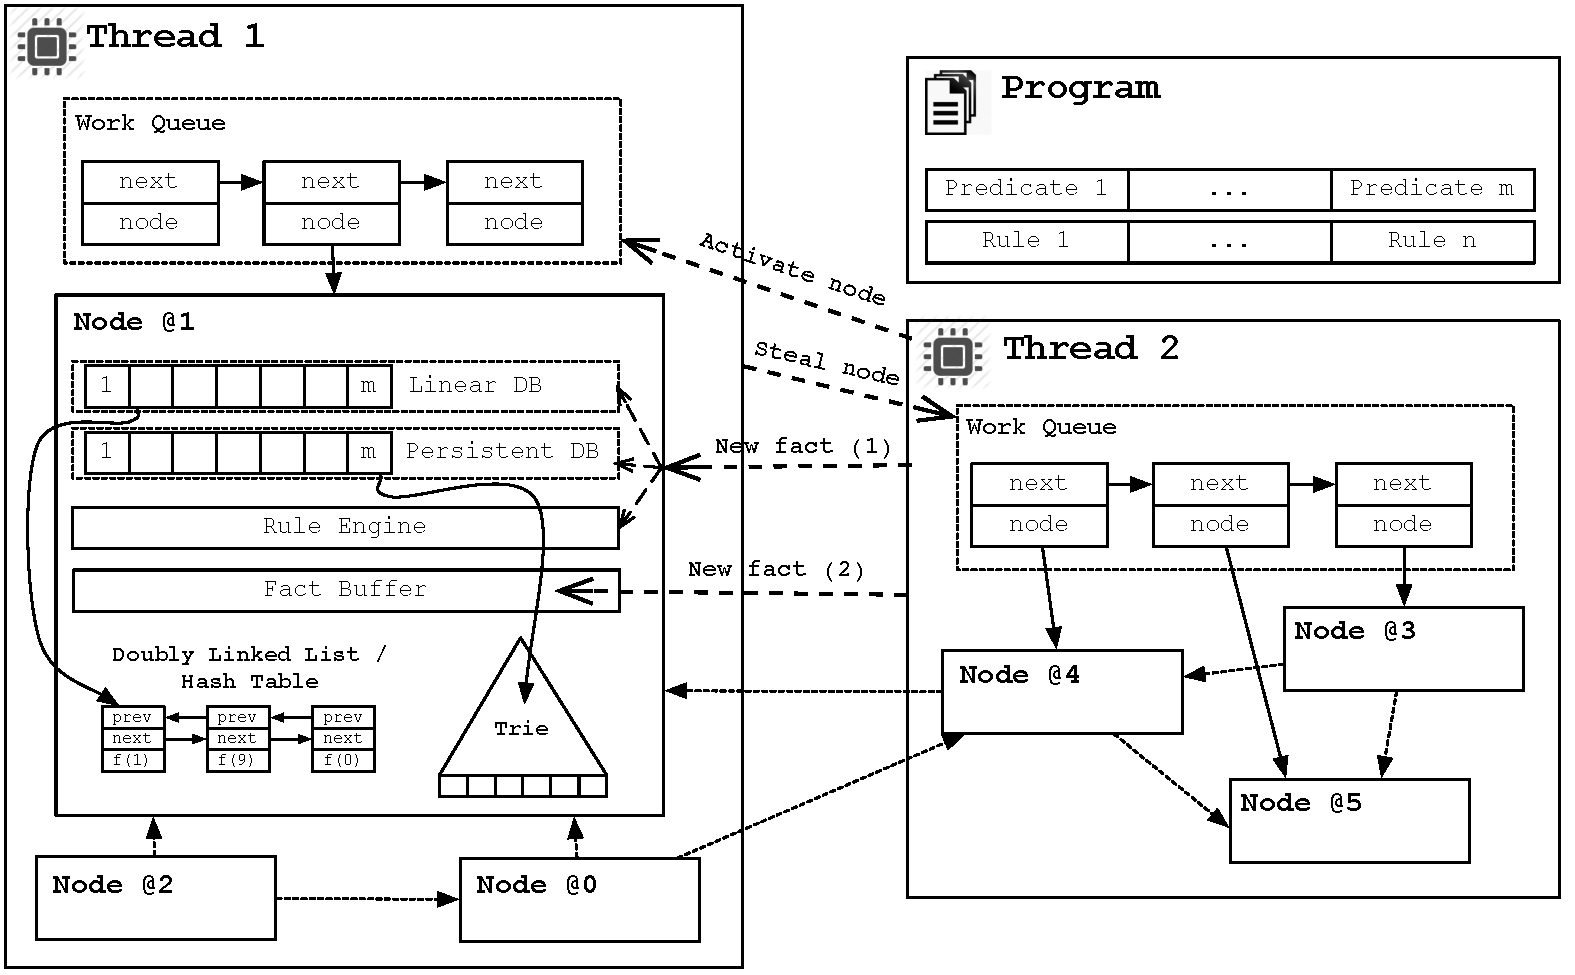
\includegraphics[width=\textwidth]{figures/overview.pdf}
\caption{Layout of the virtual machine}
\label{fig:overview}
\end{figure*}

Figure~\ref{fig:overview} presents the layout of our virtual machine
for a program with six nodes and two running threads. Each thread
space includes the nodes owned by the thread (the dotted arrows
represent the edges between nodes) and a \emph{Work Queue}, a single
linked list containing \emph{active nodes}, i.e., nodes that have new
facts to process. Initially, the \emph{Work Queue} is filled with all
the nodes of the thread in order to derive the
axioms. Figure~\ref{fig:overview} also illustrates the internal
structure layout of a node, which includes: the database of linear
facts (\emph{Linear DB}); the database of persistent facts
(\emph{Persistent DB}); the rule matching structures (\emph{Rule
Engine}); and an auxiliary buffer for storing intermediate facts
coming from other threads (\emph{Fact Buffer}).

Whenever a new fact is derived through rule derivation, we need to
update the data structures for the corresponding node. This is trivial
if the thread that derived the fact also owns the node. If that is not
the case, then we have to synchronize since multiple threads might be
updating the same node's data structures. We added a lock and a
boolean flag to each node to protect the access to its data
structures. When the flag is activated, it means that the node is
currently being executed by the owning thread. For example, in
Fig.~\ref{fig:overview}, if thread 2 derives a fact to
node \texttt{@1} (owned by thread 1), then thread 2 checks the node's
flag and if not activated, will lock node \texttt{@1} and perform the
required updates (\emph{New fact (1)}). If the flag is activated, it
will not touch the main node data structures, but instead will add the
new fact to \emph{Fact Buffer} (\emph{New fact (2)}). The facts stored
in \emph{Fact Buffer} will then be processed whenever the
corresponding node's flag becomes active.

There is another thread interaction that might happen during fact
derivation if the node receiving a new fact is not active. In such
case, the sending thread needs to activate the node by pushing it to
the \emph{Work Queue} of the target thread. For example, consider
again the situation in which thread 2 sends a new fact to
node \texttt{@1}. If node \texttt{@1} is not active, then thread 2
also needs to activate it by pushing it to the \emph{Work Queue} of
thread 1. After this synchronization point, if the target thread is
currently idle, it will become active and with a new node to process.


\subsection{Database Data Structures}
\label{sec:database}

We said before that LM rules are constrained by the first argument and
that each node has its own database of linear and persistent
facts. Moreover, since only one thread at a time will be using a
node's database, we do not need to deal with synchronization
issues. Note also that the first argument of each fact is not stored.

The database must be implemented efficiently because during matching
of rules we need to restrict the facts using a given \emph{match
object}, which fixes arguments of the target predicate to instantiated
values. Each node's database is implemented using three kinds of data
structures:

\begin{itemize}
\item \emph{Trie Data Structures} are used exclusively to store 
  persistent facts. Tries are trees where facts are indexed by common
  prefix arguments.
\item \emph{Doubly Linked List Data Structures} are used to store 
  linear facts. We use a double linked list because it is a very
   efficient way to add and remove facts.
\item \emph{Hash Table Data Structures} are used to improve lookup when 
  linked lists are too long and when we need to do search filtered by
  a fixed argument. The virtual machine decides which arguments are
  best to be indexed (see Section~\ref{indexing}) and then uses a hash table
  indexed by the appropriate argument. If we need to go through all
  the facts, we just iterate through all the facts in the table. For
  collisions, we use the above doubly linked list data structure.
\end{itemize}

Figure~\ref{fig:hash_table} shows an example for a hash table data
structure for a \texttt{a(int,int)} predicate with 3 linear facts
indexed by the second argument and stored as a doubly linked list in
bucket \texttt{2}. Each linear fact contains the regular list
pointers, a \texttt{flags} field and the fact arguments. Those are all
stored continuously to improve data locality. One use of
the \texttt{flags} field is to mark that a fact is already being
used. For example, consider the rule:

{\footnotesize
\begin{Verbatim}
a(A,B), a(C,D) -o ...
\end{Verbatim}
}

When we first pick a fact for \texttt{a(A, B)} from the hash
table, we mark it as being used in order to ensure that, when we
retrieve facts for \texttt{a(C, D)}, the first one cannot be used
twice since that would violate linearity.

\begin{figure}[ht]
\centering
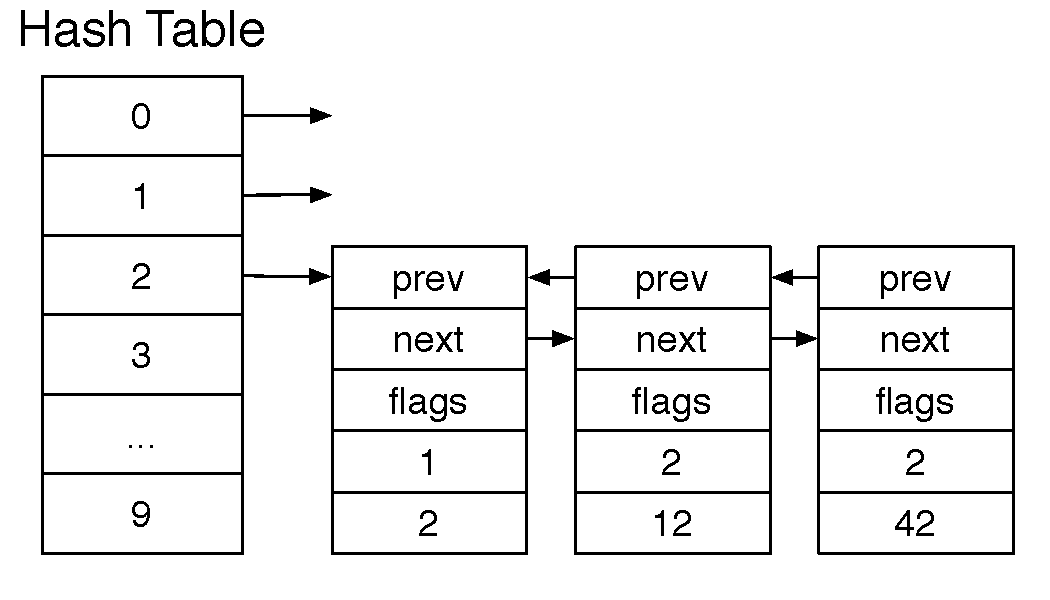
\includegraphics[width=0.4\textwidth]{figures/hash_table.pdf}
\caption{Hash table and doubly linked data structures for 
  a \texttt{a(int,int)} predicate}
\label{fig:hash_table}
\end{figure}


\subsection{Rule Engine}
\label{rule_engine}

The rule engine decides which rules may need to be executed while
taking into account rule priorities. Figure~\ref{fig:rule_engine}
shows the rule engine data structures in more detail. There are 4 main
data structures for scheduling rule execution: \texttt{Rule Queue} is
the bitmap representing the rules scheduled to run; \texttt{Active
Bitmap} contains the rules that have enough facts to be
fired; \texttt{Dropped Bitmap} contains the rules that must be dropped
from \texttt{Rule Queue} and \texttt{Active Bitmap} if the rule being
executed succeeds; and \texttt{Predicates Count} counts the number of
facts per predicate. To understand how our engine works, consider the
following set of facts and rules:

{\footnotesize
\begin{Verbatim}
a.
e(0).

a, e(1) -o b.  // rule 1
a -o c.        // rule 2
b -o d.        // rule 3
e(0) -o f.     // rule 4
c -o e(1).     // rule 5
\end{Verbatim}
}

\begin{figure*}[t]
\centering
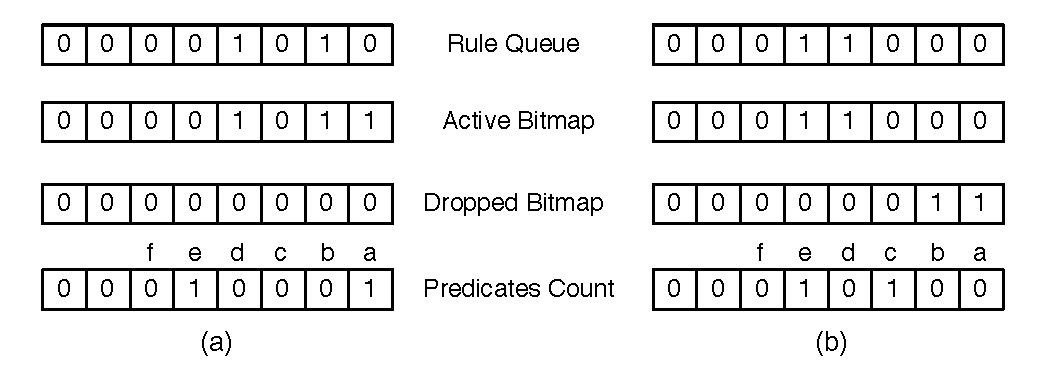
\includegraphics[width=11cm]{figures/rule_queue.pdf}
\caption{Rule engine data structures (a) before and (b) after applying 
  the rule \texttt{a -o c.}}
\label{fig:rule_engine}
\end{figure*}

Since we have facts for predicates \texttt{a/0} and \texttt{e/1},
the \texttt{Active Bitmap} starts with rules 1, 2 and 4 marked as
having enough facts to be fired. The \texttt{Rule Queue} bitmap also
starts with the same three rules. In order to pick rules for
execution, we take the rule corresponding to the least significant bit
from the \texttt{Rule Queue} bitmap, initially the first
rule \texttt{a, e(1) -o b}. However, since we don't have
fact \texttt{e(1)}, this rule fails and we execute the second
rule \texttt{a -o c}. Figure~\ref{fig:rule_engine}(a) shows the rule
engine data structures at that point.

Because the derivation for the second rule succeeds, we will consume
fact \texttt{a} and derive fact \texttt{c}. We thus update
\texttt{Predicates Count} accordingly, mark the first 
and second rules in \texttt{Dropped Bitmap} since such rules are no
longer applicable (\texttt{a} was consumed) and mark the fifth rule
in \texttt{Active Bitmap} since \texttt{c} was derived. Finally, to
update the \texttt{Rule Queue}, we remove the bits marked
in \texttt{Dropped Bitmap} and add the active rules marked
in \texttt{Active Bitmap} that use the newly derived predicates, rule
5 in this case. In the continuation, the engine will schedule the
fourth and fifth rules to run. Figure~\ref{fig:rule_engine}(b) shows
the rule engine data structures at that point.

Note that every node in the program has the same set of data
structures presented in Fig.~\ref{fig:rule_engine}. We use 32 bits
integers to implement the 3 bitmaps and an array of 16 bits integers to
count facts.

We do a small optimization to reduce the number of derivations of
persistent facts and, for that, we divide the program rules into two
sets: \emph{persistent rules} and \emph{non persistent rules}.
Persistent rules are rules where only persistent facts are
involved. We compile such rules incrementally, i.e., we attempt to
fire all rules where a persistent fact is used. This is called
the \emph{pipelined semi-naive} evaluation and it originated in the P2
system~\cite{Loo-condie-garofalakis-p2}. This evaluation method avoids
excessing re-derivations of the same fact. The order of derivation
does not matter for those rules, since only persistent facts are used.


\subsection{Rule Execution}

A byte-code file contains meta-data about the program's predicates,
initial nodes, partitioning information, and code for each rule. Each
VM thread has 32 registers that are used during rule
execution. Registers can store facts, integers, floats, node addresses
and pointers to runtime data structures (lists and structures). When
registers store facts, we can reference fields in the fact through the
register.

Consider the example in Fig.~\ref{fig:byte_code} that shows the LM
byte-code for the rule \texttt{!a(X,Y), b(X,Z), c(X,Y) -o
d(Y)}. Consider also a database with the
facts \texttt{!a(1,2)}, \texttt{!a(2,3)}, \texttt{b(1,3)},
\texttt{b(5,3)}, \texttt{c(1,2)}, \texttt{c(1,3)}, \texttt{c(5,3)}. Rule
execution for this rule and facts proceeds in a series of recursive
loops, as follows. The first loop retrieves an iterator for the
persistent facts of \texttt{!a/2} and moves the first valid
fact, \texttt{!a(1,2)}, to register 0. The inner loop retrieves linear
facts that match \texttt{b(1,Z)} (from the
\emph{join constraint}) and moves \texttt{b(1,3)} to register 1. The 
final loop moves \texttt{c(1,2)} to register 2 and the body of the
rule is successfully matched. Next, we derive \texttt{d(2)},
where \texttt{2} comes from register 0.

\begin{figure}[ht]
{\footnotesize
\begin{Verbatim}
PERSISTENT ITERATE a MATCHING TO reg 0
   LINEAR ITERATE b MATCHING TO reg 1
      (match).0=0.0                  // match argument X
      LINEAR ITERATE c MATCHING TO reg 2
         (match).0=0.0               // match argument X
         (match).1=0.1               // match argument Y
         ALLOC d TO reg 3
         MVFIELDFIELD 0.1 TO 3.0       // get argument Y
         ADDLINEAR reg 3                  // derive d(Y)
         REMOVE reg 2
         REMOVE reg 1
         TRY NEXT
      NEXT
   NEXT
RETURN
\end{Verbatim}
}
\caption{LM byte-code for rule \texttt{!a(X,Y), b(X,Z), c(X,Y) -o d(Y)}}
\label{fig:byte_code}
\end{figure}

In case of failure, we jump to the previous loop in order to try the
next candidate fact. In case of rule success, the head is derived and
we should backtrack to the inner most \emph{valid loop}, i.e., the
older loop that uses linear facts or, if there are no linear facts
involved, to the previous loop. We need to jump to a valid loop
because we may have loops with linear facts that are now invalid. In
our example, we would jump to the loop of \texttt{b(X,Z)} and
not \texttt{c(X,Y)}, since \texttt{b(1,3)} was consumed.

As an optimization, the compiler re-orders the fact expressions used
in the body in order to make execution more efficient. For example, it
forces the join constraints in rules to appear first so that matching
will fail sooner rather than later. It also does the same for
constraints. Note also that for every loop, the compiler adds
the \emph{match object}, which contains information about which
arguments need to match, so that runtime matching be efficient.

Our compiler also detects cases where we re-derive a linear fact with
new arguments. For example, as shown in Fig.~\ref{code:update}, the LM
byte-code for rule \texttt{a(N) -o a(N+1)} will compile to code that
reuses/updates the old \texttt{a(N)} fact when deriving the
new \texttt{a(N+1)} fact.

\begin{figure}[ht]
{\footnotesize
\begin{Verbatim}
LINEAR ITERATE a MATCHING TO reg 0
   MVFIELDREG 0.0 TO reg 1           // initial argument
   MVINTREG INT 1 TO reg 2
   reg 1 INT PLUS reg 2 TO reg 3
   MVREGFIELD reg 3 TO 0.0      // reuse/update argument
   UPDATE reg 0
   TRY NEXT
RETURN
\end{Verbatim}
}
\caption{\small{LM byte-code for rule \texttt{a(N) -o a(N+1)}}}
\label{code:update}
\end{figure}


\subsection{Indexing}
\label{indexing}

To improve fact lookup, the VM employs a fully dynamic mechanism to
decide which argument may be optimal to index.  The algorithm is
performed in the beginning of the execution and empirically tries to
assess the argument of each predicate that more equally spreads the
database across the values of the argument.  A single thread performs
the algorithm for all predicates.

The indexing algorithm is performed in three main steps. First, it
gathers statistics of lookup data by keeping a counter for each
predicate's argument.  Every time a fact search is performed where
arguments are fixed to a value, the counter of such arguments is
incremented. This phase is performed during rule execution for a small
fraction of the nodes in the program.

The second step of the algorithm then decides the candidate arguments
of each predicate.  If a predicate was not searched with any fixed
arguments, then it will be not indexed.  If only one argument was
fixed, then such argument is set as the indexing argument. Otherwise,
the top 2 arguments are selected for the third phase,
where \emph{entropy statistics} are collected dynamically.

During the third phase, each candidate argument has an entropy score.
Before a node is executed, the facts of the target predicate
are used in the following formula applied for the two arguments:

{\tiny
\[
Entropy(A, F) = - \sum_{v \in values(F, A)} \frac{count(F, A = v)}{total(F)} \log_2 \frac{count(F, A = v)}{total(F)}
\]
}

\noindent
where $A$ is the target argument, $F$ is the set of linear facts
for the target predicate, $values(F, A)$ is set of values of the
argument $A$, $count(F, A = v)$ counts the number of linear facts
where argument $A$ is equal to $v$ and $total(F)$ counts the number of
linear facts in $F$.  The entropy value is a good metric because it
tells us how much information is needed to describe an argument.  If
more information is needed, then that must be the best argument to
index.

For one of the arguments to score, $Entropy(A, F)$ multiplied by the
number of times it has been used for lookup must be larger than the
other argument. The argument with the best score is selected and then
a global variable called \texttt{indexing\_epoch} is updated.  In
order to convert the node's linked lists into hash tables, each node
also has a local variable called \texttt{indexing\_epoch} that is
compared to the global variable in order to rebuild the node database
according to the new indexing information.

Our VM also dynamically resizes the hash table if necessary. When the
hash table becomes too dense, it is resized to the double. When it
becomes too sparse, it is reduced in half or simply transformed back
into a doubly linked list. This is done once in a while, before a node
executes.

We have seen very good results with this scheme. For example, for the
all-pairs shortest paths program, we obtained a 2 to 5-fold
improvement in sequential execution time.  The overhead of dynamic
indexing is negligible since programs run almost as fast as if the
indices have been added from the start.


\subsection{Runtime Data Structures}

LM also supports recursive types such as lists and pairs. These
complex data structures are stored in the heap of the VM and are
managed through reference counting. For instance, each list is
a \emph{cons cell} with 3 fields: \texttt{tail}, the pointer to the
next element of the list; \texttt{head}, the element stored by this
element of the list; and \texttt{refs} that counts the number of
pointers to this list element in the VM. The list is deleted from the
heap whenever \texttt{refs} is decremented to zero.

We avoid garbage collection schemes since objects are created and discarded
in very specific points of the virtual machine and our objects cannot contain circular references.
A reference counting mechanism is thus more appropriate than a parallel garbage collector which
would entail pausing the execution of the program to garbage collect all the unused objects.
 
\makeatletter{}\newcommand{\plotsize}{0.45\textwidth}


\section{Experimental Results}
\label{results}

This section presents initial results for our VM. First, we present a
comparison with similar programs written in other programming
languages in order to show evidence that our VM is viable. Then, we
present scalability results in order to show that LM programs can take
advantage of multicore architectures.

For our experimental setup, we used a machine with 32 (2x16) Core AMD
Opteron (tm) Processor 6274 $@$ 2.2 GHz with 32 GBytes of RAM memory
and running the Linux kernel 3.8.3-1.fc17.x86\_64.  We compiled our VM
using GCC 4.7.2 (g++) with the flags \texttt{-O3 -std=c+0x
  -march=x86-64}. We run all experiments 3 times and averaged the
execution time.


\subsection{Absolute Execution Time}

To put our VM in perspective, we first compare it in terms of absolute
execution time with other competing systems using a single thread.

In Table~\ref{tbl:comp_nqueens}, we compare LM's version of the
classic N-Queens puzzle against 3 other versions: a straightforward
sequential program implemented in C using backtracking; a sequential
Python implementation~\cite{vanRossum:1995:PRM}; and a Prolog
implementation executed in YAP
Prolog~\cite{DBLP:journals/corr/abs-1102-3896}, an efficient
implementation of Prolog. Numbers less than 1 mean that LM is faster
and larger than 1 mean that LM is slower. We can observe that LM
easily beats Python, but is 5 to 10 times slower than YAP Prolog and
around 15 times slower than C. Note however that, as we will see next,
if we use at least 16 threads in LM, we can beat the sequential
implementation written in C.

\begin{table}[ht]
\centering
{\begin{tabular}{c|c|c|c}
\textbf{Problem} & \multicolumn{3}{c}{\textbf{System}} \\
\textbf{Size} & \textbf{C} & \textbf{Python} & \textbf{YAP Prolog} \\
\hline\hline
\textbf{10x10} & 16.92 & 0.62 & 5.42 \\
\textbf{11x11} & 21.59 & 0.64 & 6.47 \\
\textbf{12x12} & 10.32 & 0.73 & 7.61 \\
\textbf{13x13} & 14.35 & 0.88 & 10.38 \\
\end{tabular}}
\caption{Comparing the absolute execution times (LM/System) for the
  N-Queens program}
\label{tbl:comp_nqueens}
\end{table}

In Table~\ref{tbl:comp_bp}, we compare LM's Belief Propagation (BP)
program, a machine learning algorithm to denoise images, against a
sequential C, Python and GraphLab~\cite{GraphLab2010} version of the
algorithm. GraphLab is a parallel C++ library used to solve
graph-based problems in machine learning. C and GraphLab perform about
the same since they are both compiled to machine code, although
the GraphLab version is highly optimized to run on multicore architectures.
Python runs very slowly since it is a
dynamic programming language and BP has many mathematical
computations. We should note, however, that LM's version uses some
external functions written in C++ in order to improve execution time,
therefore the comparison is not totally fair.

\begin{table}[ht]
\centering
{\begin{tabular}{c|c|c|c}
\textbf{Problem} & \multicolumn{3}{c}{\textbf{System}} \\
\textbf{Size} & \textbf{C} & \textbf{Python} & \textbf{GraphLab} \\
\hline\hline
\textbf{10}  & 1.00 & 0.03 & 1.00 \\
\textbf{50}  & 1.77 & 0.04 & 1.73 \\
\textbf{200} & 1.99 & 0.05 & 1.79 \\
\textbf{400} & 2.00 & 0.04 & 1.80 \\
\end{tabular}}
\caption{Comparing the absolute execution times (LM/System) for the
  Belief Propagation program}
\label{tbl:comp_bp}
\end{table}

We also compared a LM's version of the PageRank program against a
similar GraphLab version and LM showed to be around 4 to 6 times
slower. Our worse results were obtained for the all-pairs shortest
distance algorithm where a LM's version of the problem was around 50
times slower than a C sequential implementation of the Dijkstra
algorithm, but almost twice as fast when compared to the same
implementation in Python.


\subsection{Scalability}

\begin{figure*}[ht]
\centering
\subfigure[PageRank using a graph of web pages with around 12,000 nodes and 292,000 edges]
   {\label{exp:pagerank}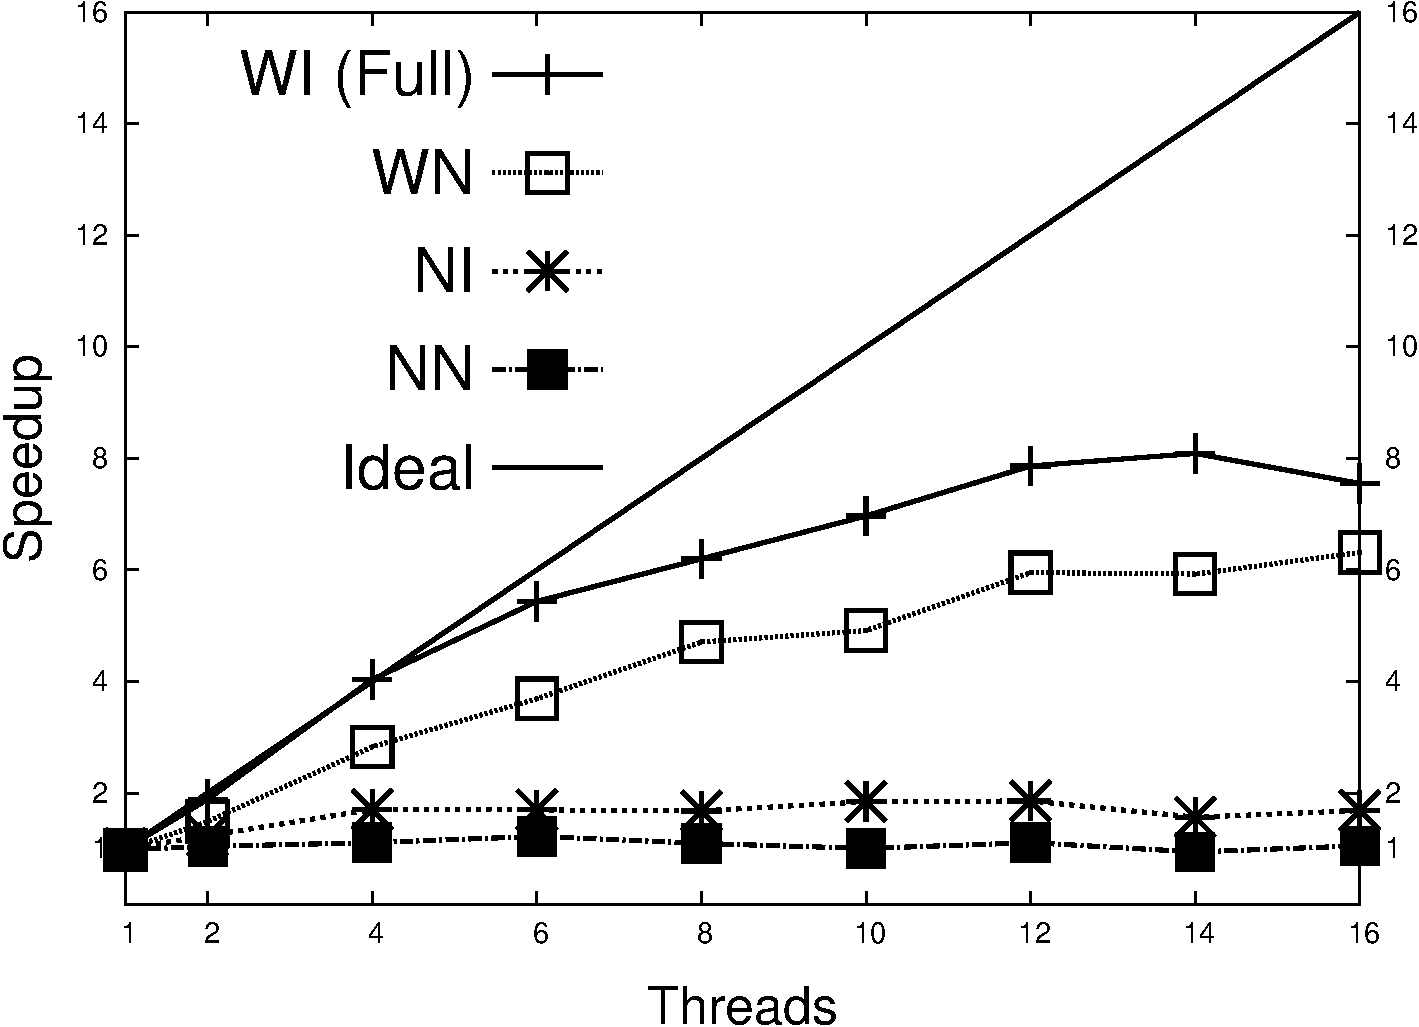
\includegraphics[width=\plotsize]{figures/results-pagerank-search-engines.pdf}}
\hspace{0.5cm}
\subfigure[GGC using a random graph with 2,000 nodes and 600,000 edges]
   {\label{exp:ggc}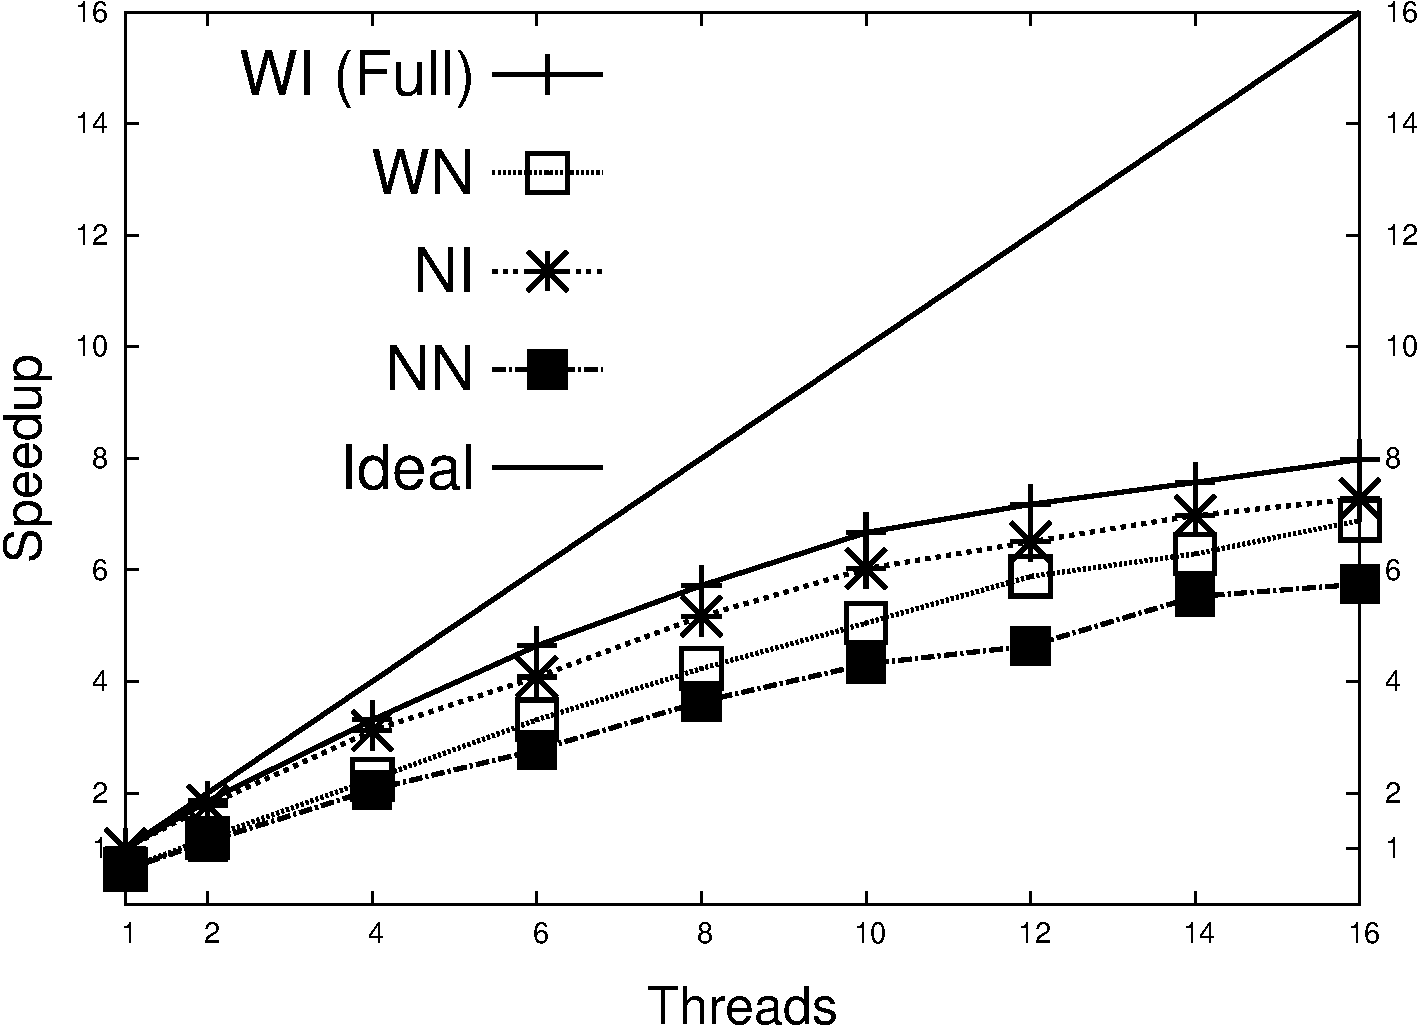
\includegraphics[width=\plotsize]{figures/results-ggc.pdf}}
\caption{Experimental results for the PageRank and GGC  algorithms}
\end{figure*}

\begin{figure*}[ht]
\centering
\subfigure[Shortest Distance for a graph with around 5,000 nodes and 13,000 edges]
   {\label{exp:sd}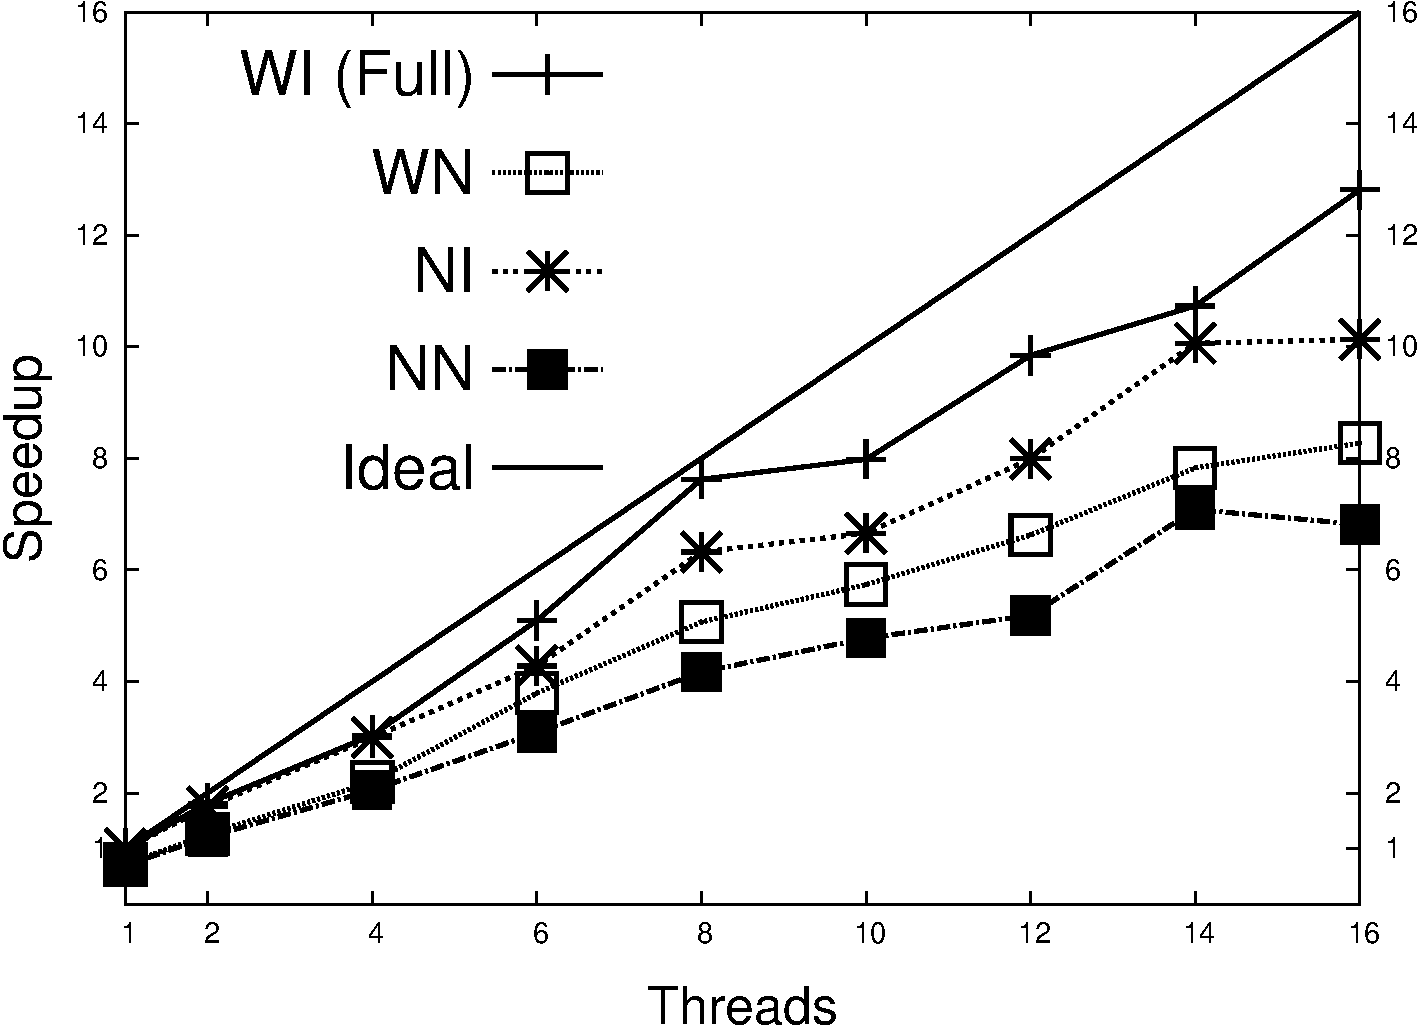
\includegraphics[width=\plotsize]{figures/results-shortest-uspowergrid.pdf}}
\hspace{0.5cm}
\subfigure[MiniMax algorithm for the Tic-Tac-Toe game (complete tree)]
   {\label{exp:minimax}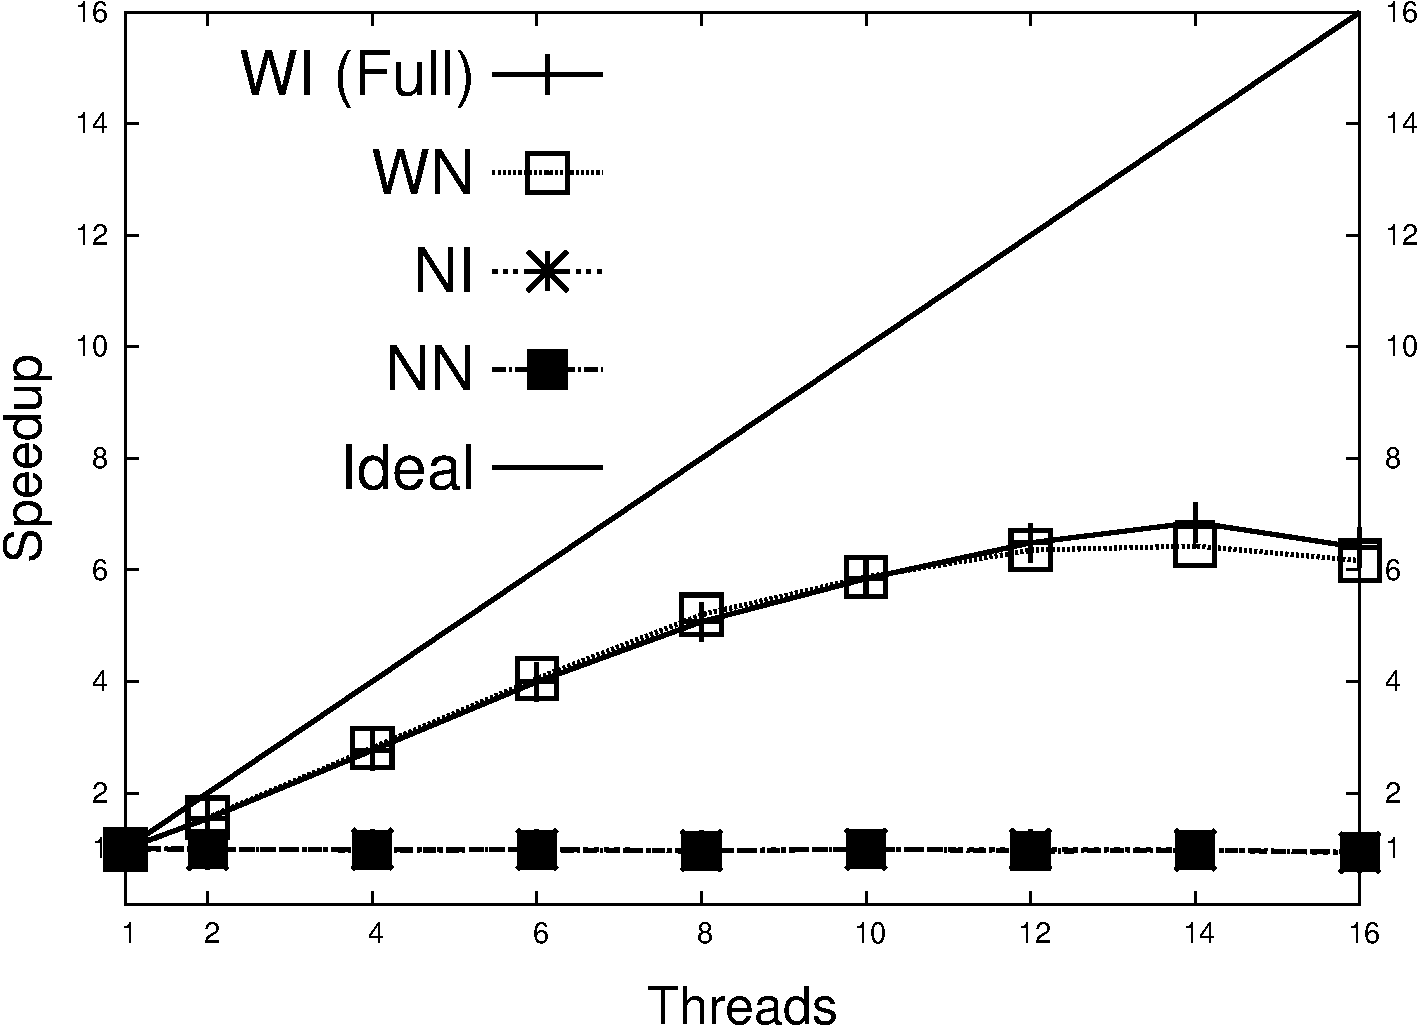
\includegraphics[width=\plotsize]{figures/results-minimax.pdf}}
\caption{Experimental results for the Shortest Distance and MiniMax algorithm}
\end{figure*}

\begin{figure*}[ht]
\centering
\subfigure[N-Queens program (13x13~board)]
   {\label{exp:13queens}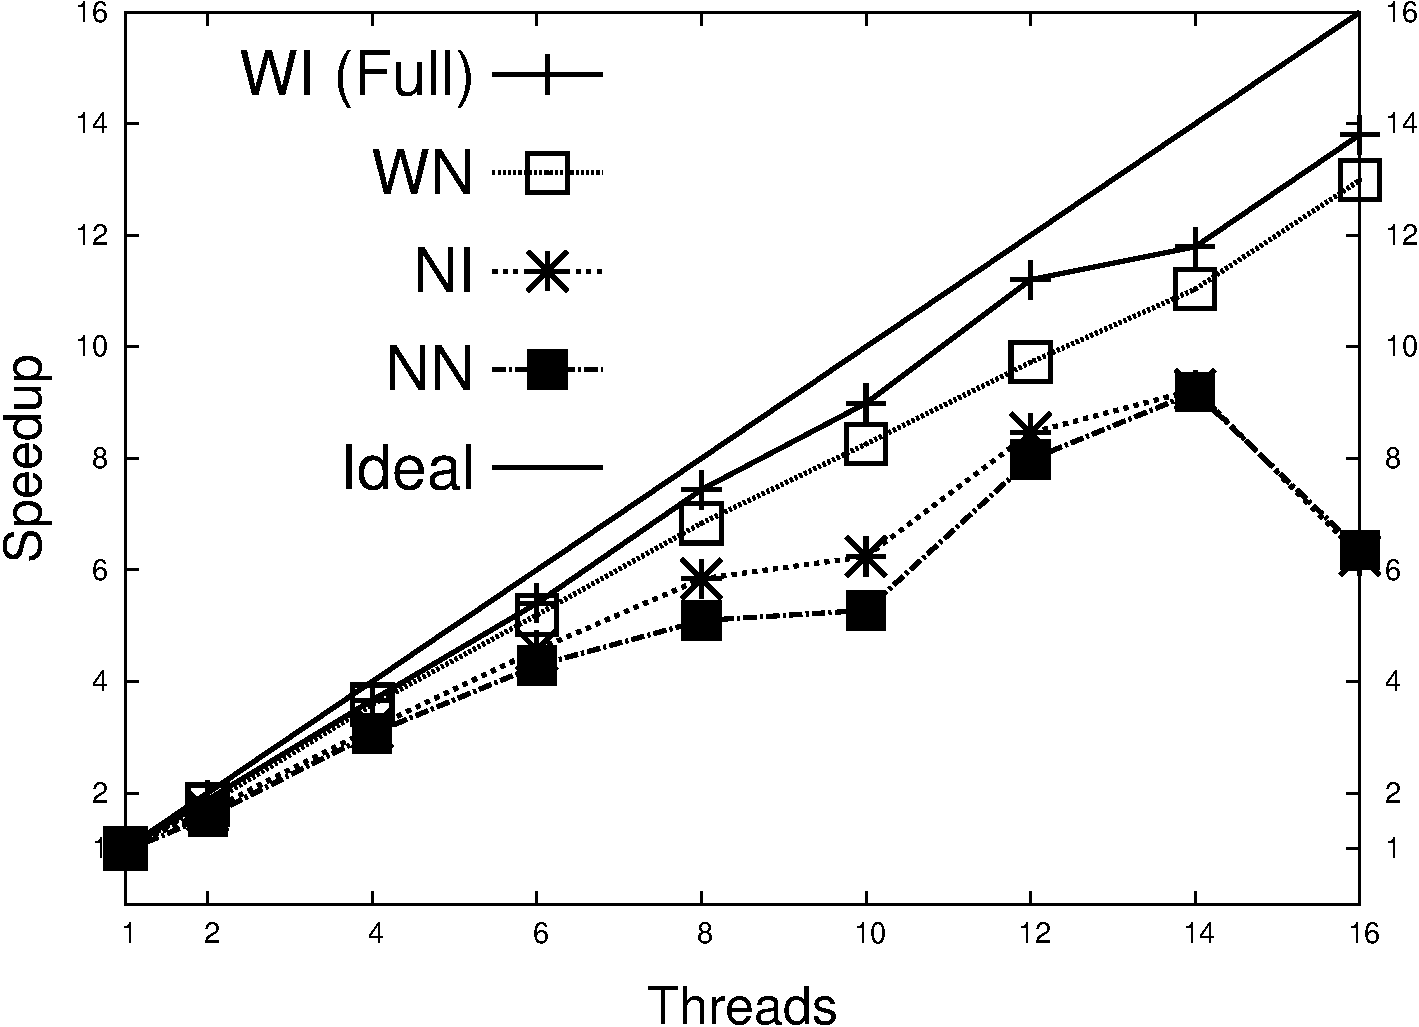
\includegraphics[width=\plotsize]{figures/results-13queens.pdf}}
\hspace{0.5cm}
\subfigure[Belief Propagation (400x400~image)]
   {\label{exp:bp}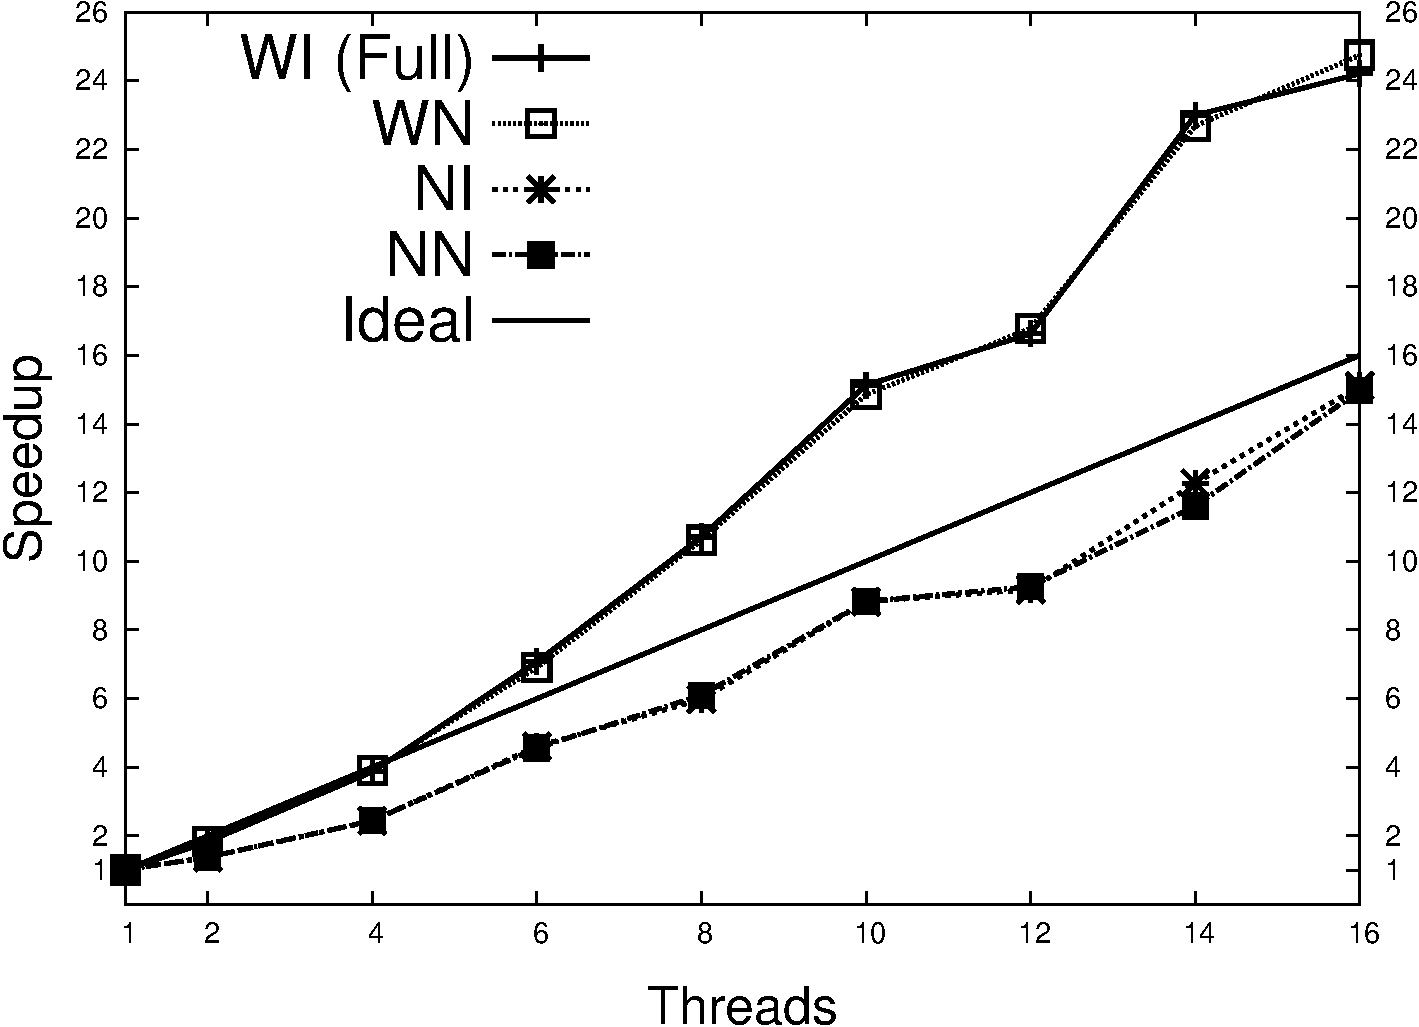
\includegraphics[width=\plotsize]{figures/results-bp.pdf}}
\caption{Experimental results for the N-Queens and Belief Propagation programs}
\end{figure*}

In this section we measure the scalability of the VM along with the
performance gains due to work stealing and dynamic indexing.  For
this purpose, we used 4 configurations for the VM: \textbf{WI}, the
full configuration that includes work stealing and dynamic indexing;
\textbf{WN}, with work stealing but without dynamic
indexing; \textbf{NI}, with indexing but without work stealing; and
\textbf{NN}, without work stealing and without dynamic indexing.  We
ran each configuration using 1, 2, 4, 6, 8, 10, 12, 14 and 16 threads
and compared the run time against the sequential execution (1 thread)
of \textbf{WI}. We used the following set of programs:

\begin{itemize}
\item PageRank implements a PageRank algorithm without synchronization
  between iterations. Every time a node sends a new rank to its
  neighbors and the change was significant, the neighbors are
  scheduled to recompute their ranks.
\item Greedy Graph Coloring (GGC) colors nodes in a graph so that no
  two adjacent nodes have the same color. We start with a small number
  of colors and then we expand the number of colors when we cannot
  color the graph.
\item Shortest Distance (SD) computes the shortest distance of all
  nodes to all nodes.
\item MiniMax, the AI algorithm for selecting the best player move in a game of Tic-Tac-Toe.
\item N-Queens, the classic puzzle for a 13x13 board.
\item Belief Propagation, a machine learning algorithm to denoise
  images.
\end{itemize}

The PageRank results are shown in Fig.~\ref{exp:pagerank}. We used a
search engine graph of 12,000 webpages\footnote{Available from
  \url{http://www.cs.toronto.edu/~tsap/experiments/download/download.html}}. Since
this dataset follows the power law, that is, there is a small number
of pages with a lots of links (1\% of the nodes have 75\% of the
edges), it can be difficult to parallelize. Our results show that the
VM is able to scale the program with up to 14 threads.  We also notice
the huge performance drop when we run the VM without work
stealing. Dynamic indexing is also an advantage, since it detects that
the facts for the pagerank of neighboring nodes need to be indexed
efficiently.

Figure~\ref{exp:ggc} presents the results for the GGC program with a
random dataset of 2,000 nodes with an uniform distribution of edges.
There is a slight drop in scalability as the number of threads goes
up, but the VM is still capable of reducing the run time. We note that
in this program, the work available is reduced as the graph becomes
increasingly colored.

In Fig.~\ref{exp:sd} we show the results for the Shortest Distance program.
We attain a 13-fold speedup for 16 threads with both work stealing and dynamic
indexing (\textbf{WI}). We note that indexing is more advantageous than work stealing
because indexing the distance facts according to the source node is more crucial
than improved load balancing.

The results for the MiniMax algorithm are presented in Fig.~\ref{exp:minimax}.
MiniMax is very different than the other algorithms because the graph of nodes is dynamic
and is created during program execution. The load balancing is also problematic since there
is little work to do in the initial and final phases of the algorithm. Still, our VM has decent
performance, with almost a 7-fold speedup for 14 threads. The scalability drops with 16 threads
but we think that is due to the simplicity of the current work stealing algorithm.
Dynamic indexing has no effects in this program.

The results for the N-Queens program are shown in
Fig.~\ref{exp:13queens}. The program is not regular since computation
starts at the top of the grid and then rolls down, until only the last
row be doing computation. Because the number of valid states for the
nodes in the upper rows is much less than the nodes in the lower rows,
this may potentially lead to load balancing problems. The results show
that our system is able to scale well. When work stealing is left out
(\textbf{NI} and \textbf{NN}), we see a serious drop in performance with 16 threads.

Finally, we shown the results for the Belief Propagation~(BP) program
in Fig.~\ref{exp:bp}. BP is a regular and asynchronous program and
benefits (as expected) from having multiple threads executing since
the belief values of each node will converge faster.  The super-linear
results prove this assertion.

\subsection{Memory Statistics}

In this section, we present the amount of memory used by the VM after the
programs presented in the previous section complete. We also count the number of
facts stored in the database. This serves as an indication of
how much memory is needed in terms of the number of facts stored in the database.
Results are shown in Table~\ref{tbl:memory}.

\begin{table}[ht]
\centering
{\begin{tabular}{c|c|c|c}
\textbf{Program} & \textbf{Facts} & \textbf{Memory} & \textbf{Per Fact} \\
\hline\hline
PageRank & 1,180,603 & 203,832 KB & 176 bytes \\
GGC & 2,363,536 & 292,682 KB & 127 bytes \\
SD & 502,347 & 45,387 KB & 92 bytes \\
MiniMax & 3 & 886,443 KB & 295,481 KB \\
N-Queens & 74,557 & 55,408 KB & 760 bytes \\
BP & 2,235,200 & 617,417 KB & 283 bytes \\
\hline\hline
\multicolumn{3}{l}{Average (without MiniMax) } & 288 bytes \\
\end{tabular}}
\caption{Memory usage of programs after completion using 1 thread.}
\label{tbl:memory}
\end{table}

The most unexpected result in Table~\ref{tbl:memory} is that of the MiniMax program. There is a
very low number of facts (that indicate the final player decision) and a huge
amount of memory. How can this be explained? We note that MiniMax builds a huge
decision tree of nodes with almost $9!$ leaves. Although these nodes do not participate
in the computation after the MiniMax result is computed for them, the VM does not garbage collect
nodes that do not contain facts and that do not have external references from other nodes.
This is a potential improvement that can be done in the future.

PageRank, GGC and SD show a low memory usage per fact. This makes sense since the predicates
used in those programs are relatively simple with only a few arguments.
This changes with the N-Queens problem where the predicates have lists representing the valid
positions of the queens in the board. Storing lists is far more expensive than storing integral
values such as integers or floating point numbers. The same happens with BP because
the belief values are stored as lists of floating point numbers.
 
\makeatletter{}\section{Related Work}
\label{related_work}

Virtual machines are a popular technique for implementing interpreters
for high level programming languages.  Due to the increased
availability of parallel machines and distributed architectures,
several machine models have been developed with parallelism in
mind~\cite{Kara:1997:AMM:265274}.  One example of such machine is the
Parallel Virtual Machine (PVM)~\cite{Sunderam90pvm:a}, which serves as
an abstraction to program heterogeneous computers as a single
machine. Another important machine is the Threaded Abstract Machine
(TAM)~\cite{CullerGSvE93,goldstein-tr94}, which defines a
self-scheduled machine language of parallel threads where a program is
represented as conventional control flow.

Prolog, the most prominent logic programming language, has a rich
history of virtual machine research centered around the Warren
Abstract Machine (WAM)~\cite{AICPub641:1983}. 
Prolog is naturally parallel because several clauses for the same goal
(AND-parallelism) or all goals in a clause (OR-parallelism) can be
tried in parallel. Different abstract machines for AND-parallelism has
been developed on top of the
WAM~\cite{Hermenegildo:1986:AMB:913061,Lin:1988:AEL:900478}.  For
OR-parallelism we have several models such as: the SRI
model~\cite{Warren:1987:OEM:67683.67699}, the Argonne
model~\cite{ButlerDLOOS88}, the MUSE model~\cite{Ali:1990fk} and the
BC machine~\cite{Ali88}. While all those models have been developed
using the WAM, there are also some parallel machines totally different
from the WAM, such as the PPAM~\cite{Kacsuk:1990:EMP:533578}, which is
based on a data-flow model.

Several linear logic programming languages have been developed in the past~\cite{Miller85anoverview}.
Lolli, a programming language based on a fragment of intuitionistic linear logic~\cite{Hodas94logicprogramming}, 
proves goals by lazily managing the context of linear resources during backward-chaining proof search.
LolliMon~\cite{Lopez:2005:MCL:1069774.1069778} is a concurrent linear logic programming language that integrates
both forward and backward-chaining search, where the backward-chaining phase is done sequentially but
the forward-chaining is done concurrently inside a monad. The backward-chaining phase is suspended
between the forward-chaining phases, where a fix-point is computed.
LolliMon is derived from the concurrent logical framework called CLF~\cite{Watkins:2004uq}. 
\makeatletter{}\section{Conclusions}

We have presented a parallel virtual machine for executing
forward-chaining linear logic programs, with particular focus on
thread management, code organization, fact indexing, rule execution
and database organization for fast insertion, lookup, and deletion of
linear facts. Experimental results show that our VM is able to scale
the execution of programs when run with up to 16 threads.
Our results also show the importance of having an efficient indexing mechanisms
for facts. With our dynamic indexing, the VM automatically detects which predicates
need to be indexed in order to improve performance.
Due to these and other optimizations, the VM fairs relatively well against other programming languages, including
compiled languages. Moreover, since LM programs are
concurrent by default, we can easily get better performance from the
start by executing them with multiple threads.
As further work, we want to improve parallel scalability and
take advantage of linear logic to perform whole-program
optimizations, including computing program invariants, loop detection
in rules and bypass of rule priorities.

We think that our virtual machine is an excellent starting point to make
logic programming more desirable in the data-mining, machine learning and
distributed/parallel programming community. Moreover, our virtual machine can
be easily extended to execute over computer networks or to execute programs on really big datasets.
In a nutshell, LM provides a concise way to describe
graph-based algorithms that can be more easily reasoned about, a clear advantage over
competing systems.
 
\makeatletter{}\acks

This work is partially funded by the ERDF (European Regional
Development Fund) through the COMPETE Programme; by FCT (Portuguese
Foundation for Science and Technology) through the Carnegie Mellon
Portugal Program and project SIBILA (NORTE-07-0124-FEDER-000059); and
by the Qatar National Research Fund under grant NPRP
09-667-1-100. Flavio Cruz is funded by the FCT grant
SFRH/BD/51566/2011.
 

\balance


\bibliographystyle{abbrvnat}


\begin{thebibliography}{35}
\providecommand{\natexlab}[1]{#1}
\providecommand{\url}[1]{\texttt{#1}}
\expandafter\ifx\csname urlstyle\endcsname\relax
  \providecommand{\doi}[1]{doi: #1}\else
  \providecommand{\doi}{doi: \begingroup \urlstyle{rm}\Url}\fi

\bibitem[Ali and Karlsson(1990)]{Ali:1990fk}
K.~Ali and R.~Karlsson.
\newblock Full prolog and scheduling or-parallelism in muse.
\newblock \emph{International Journal of Parallel Programming}, 19\penalty0
  (6):\penalty0 445--475, 1990.
\newblock ISSN 0885-7458.
\newblock \doi{10.1007/BF01397627}.
\newblock URL \url{http://dx.doi.org/10.1007/BF01397627}.

\bibitem[Ali(1988)]{Ali88}
K.~A.~M. Ali.
\newblock Or-parallel execution of prolog on bc-machine.
\newblock In R.~A. Kowalski and K.~A. Bowen, editors, \emph{ICLP/SLP}, pages
  1531--1545. MIT Press, 1988.
\newblock ISBN 0-262-61056-6.
\newblock URL \url{http://dblp.uni-trier.de/db/conf/iclp/iclp88.html#Ali88}.

\bibitem[Ashley-Rollman et~al.(2007)Ashley-Rollman, Rosa, Srinivasa, Pillai,
  Goldstein, and Campbell]{ashley-rollman-derosa-iros07wksp}
M.~P. Ashley-Rollman, M.~D. Rosa, S.~S. Srinivasa, P.~Pillai, S.~C. Goldstein,
  and J.~D. Campbell.
\newblock Declarative programming for modular robots.
\newblock In \emph{Workshop on Self-Reconfigurable Robots/Systems and
  Applications at IROS 2007}, 2007.

\bibitem[Ashley-Rollman et~al.(2009)Ashley-Rollman, Lee, Goldstein, Pillai, and
  Campbell]{ashley-rollman-iclp09}
M.~P. Ashley-Rollman, P.~Lee, S.~C. Goldstein, P.~Pillai, and J.~D. Campbell.
\newblock A language for large ensembles of independently executing nodes.
\newblock In \emph{International Conference on Logic Programming (ICLP)}, 2009.

\bibitem[Baelde(2012)]{Baelde:2012:LGF:2071368.2071370}
D.~Baelde.
\newblock Least and greatest fixed points in linear logic.
\newblock \emph{ACM Transactions on Computational Logic}, 13\penalty0
  (1):\penalty0 1--44, 2012.

\bibitem[Betz and Fr{\"u}hwirth(2005)]{Betz:2005kx}
H.~Betz and T.~Fr{\"u}hwirth.
\newblock A linear-logic semantics for constraint handling rules.
\newblock In \emph{Principles and Practice of Constraint Programming - CP
  2005}, volume 3709 of \emph{Lecture Notes in Computer Science}, pages
  137--151. 2005.

\bibitem[Butler et~al.(1988)Butler, Disz, Lusk, Olson, Overbeek, and
  Stevens]{ButlerDLOOS88}
R.~Butler, T.~Disz, E.~L. Lusk, R.~Olson, R.~A. Overbeek, and R.~L. Stevens.
\newblock Scheduling or-parallelism: An argonne perspective.
\newblock In R.~A. Kowalski and K.~A. Bowen, editors, \emph{ICLP/SLP}, pages
  1590--1605. MIT Press, 1988.
\newblock ISBN 0-262-61056-6.
\newblock URL
  \url{http://dblp.uni-trier.de/db/conf/iclp/iclp88.html#ButlerDLOOS88}.

\bibitem[Colmerauer and Roussel(1993)]{Colmerauer:1993:BP:154766.155362}
A.~Colmerauer and P.~Roussel.
\newblock The birth of prolog.
\newblock In \emph{The Second ACM SIGPLAN Conference on History of Programming
  Languages}, pages 37--52, New York, NY, USA, 1993.

\bibitem[Costa et~al.(2011)Costa, Damas, and
  Rocha]{DBLP:journals/corr/abs-1102-3896}
V.~S. Costa, L.~Damas, and R.~Rocha.
\newblock The yap prolog system.
\newblock \emph{CoRR}, abs/1102.3896, 2011.

\bibitem[Cruz et~al.(2014)Cruz, Rocha, Goldstein, and Pfenning]{cruz-iclp14}
F.~Cruz, R.~Rocha, S.~Goldstein, and F.~Pfenning.
\newblock {A Linear Logic Programming Language for Concurrent Programming over
  Graph Structures}.
\newblock \emph{Journal of Theory and Practice of Logic Programming, 30th
  International Conference on Logic Programming (ICLP 2014), Special Issue},
  14\penalty0 (4 \& 5):\penalty0 493--507, July 2014.

\bibitem[Culler et~al.(1993)Culler, Goldstein, Schauser, and von
  Eicken]{CullerGSvE93}
D.~E. Culler, S.~C. Goldstein, K.~E. Schauser, and T.~von Eicken.
\newblock {TAM --- a compiler controlled threaded abstract machine}.
\newblock \emph{Journal of Parallel and Distributed Computing}, 18:\penalty0
  347--370, July 1993.
\newblock URL \url{http://www.cs.cmu.edu/~seth/papers/CullerGSvE93.pdf}.

\bibitem[Girard(1987)]{girard-87}
J.-Y. Girard.
\newblock Linear logic.
\newblock \emph{Theoretical Computer Science}, 50\penalty0 (1):\penalty0
  1--102, 1987.

\bibitem[Goldstein(1994)]{goldstein-tr94}
S.~C. Goldstein.
\newblock The implementation of a threaded abstract machine.
\newblock Technical Report UCB/CSD-94-818, EECS Department, University of
  California, Berkeley, 1994.
\newblock URL \url{http://www.cs.cmu.edu/~seth/papers/goldstein-tr94.pdf}.

\bibitem[Gonzalez et~al.(2009)Gonzalez, Low, and
  Guestrin]{Gonzalez+al:aistats09paraml}
J.~Gonzalez, Y.~Low, and C.~Guestrin.
\newblock Residual splash for optimally parallelizing belief propagation.
\newblock In \emph{Artificial Intelligence and Statistics (AISTATS)}, 2009.

\bibitem[Gupta et~al.(2001)Gupta, Pontelli, Ali, Carlsson, and
  Hermenegildo]{Gupta:2001:PEP:504083.504085}
G.~Gupta, E.~Pontelli, K.~A.~M. Ali, M.~Carlsson, and M.~V. Hermenegildo.
\newblock Parallel execution of prolog programs: {A} survey.
\newblock \emph{ACM Transactions on Programming Languages and Systems
  (TOPLAS)}, 23\penalty0 (4):\penalty0 472--602, 2001.

\bibitem[Hermenegildo(1986)]{Hermenegildo:1986:AMB:913061}
M.~V. Hermenegildo.
\newblock \emph{An Abstract Machine Based Execution Model for Computer
  Architecture Design and Efficient Implementation of Logic Programs in
  Parallel}.
\newblock PhD thesis, 1986.
\newblock AAI8700203.

\bibitem[Hodas and Miller(1994)]{Hodas94logicprogramming}
J.~S. Hodas and D.~Miller.
\newblock Logic programming in a fragment of intuitionistic linear logic.
\newblock \emph{Information and Computation}, 110:\penalty0 32--42, 1994.

\bibitem[Holzbaur et~al.(2004)Holzbaur, de~la Banda, Stuckey, and
  Duck]{DBLP:journals/corr/cs-PL-0408025}
C.~Holzbaur, M.~J.~G. de~la Banda, P.~J. Stuckey, and G.~J. Duck.
\newblock Optimizing compilation of constraint handling rules in hal.
\newblock \emph{CoRR}, cs.PL/0408025, 2004.

\bibitem[Isard et~al.(2007)Isard, Budiu, Yu, Birrell, and
  Fetterly]{Isard:2007:DDD:1272996.1273005}
M.~Isard, M.~Budiu, Y.~Yu, A.~Birrell, and D.~Fetterly.
\newblock Dryad: distributed data-parallel programs from sequential building
  blocks.
\newblock In \emph{European Conference on Computer Systems (EuroSys)}, pages
  59--72, 2007.

\bibitem[Kacsuk(1990)]{Kacsuk:1990:EMP:533578}
P.~Kacsuk.
\newblock \emph{Execution Models of PROLOG for Parallel Computers}.
\newblock MIT Press, Cambridge, MA, USA, 1990.
\newblock ISBN 0262111497.

\bibitem[Kara et~al.(1997)Kara, Davy, Goodeve, and Nash]{Kara:1997:AMM:265274}
M.~Kara, J.~R. Davy, D.~Goodeve, and J.~Nash, editors.
\newblock \emph{Abstract Machine Models for Parallel and Distributed
  Computing}.
\newblock IOS Press, Amsterdam, The Netherlands, The Netherlands, 1997.
\newblock ISBN 90-5199-267-X.

\bibitem[Lam and Sulzmann(2010)]{DBLP:journals/corr/abs-1006-3039}
E.~S.~L. Lam and M.~Sulzmann.
\newblock Concurrent goal-based execution of constraint handling rules.
\newblock \emph{CoRR}, abs/1006.3039, 2010.

\bibitem[Lin and Kumar(1988)]{Lin:1988:AEL:900478}
Y.~Lin and V.~Kumar.
\newblock And-parallel execution of logic programs on a shared memory
  multiprocessor:a summary of results.
\newblock Technical report, Austin, TX, USA, 1988.

\bibitem[Liu(1998)]{Liu98extendingdatalog}
M.~Liu.
\newblock Extending datalog with declarative updates.
\newblock In \emph{International Conference on Database and Expert System
  Applications (DEXA)}, volume 1873, pages 752--763, 1998.

\bibitem[Loo et~al.(2006)Loo, Condie, Garofalakis, Gay, and
  Hellerstein]{Loo-condie-garofalakis-p2}
B.~T. Loo, T.~Condie, M.~Garofalakis, D.~E. Gay, and J.~M. Hellerstein.
\newblock Declarative networking: Language, execution and optimization.
\newblock In \emph{International Conference on Management of Data (SIGMOD)},
  pages 97--108, 2006.

\bibitem[L\'{o}pez et~al.(2005)L\'{o}pez, Pfenning, Polakow, and
  Watkins]{Lopez:2005:MCL:1069774.1069778}
P.~L\'{o}pez, F.~Pfenning, J.~Polakow, and K.~Watkins.
\newblock Monadic concurrent linear logic programming.
\newblock In \emph{Proceedings of the 7th ACM SIGPLAN International Conference
  on Principles and Practice of Declarative Programming}, PPDP '05, pages
  35--46, New York, NY, USA, 2005.

\bibitem[Low et~al.(2010)Low, Gonzalez, Kyrola, Bickson, Guestrin, and
  Hellerstein]{GraphLab2010}
Y.~Low, J.~Gonzalez, A.~Kyrola, D.~Bickson, C.~Guestrin, and J.~M. Hellerstein.
\newblock Graphlab: {A} new framework for parallel machine learning.
\newblock In \emph{Conference on Uncertainty in Artificial Intelligence (UAI)},
  pages 340--349, 2010.

\bibitem[Malewicz et~al.(2010)Malewicz, Austern, Bik, Dehnert, Horn, Leiser,
  and Czajkowski]{Malewicz:2010:PSL:1807167.1807184}
G.~Malewicz, M.~H. Austern, A.~J.~C. Bik, J.~C. Dehnert, I.~Horn, N.~Leiser,
  and G.~Czajkowski.
\newblock Pregel: a system for large-scale graph processing.
\newblock In \emph{International Conference on Management of Data (SIGMOD)},
  pages 135--146, 2010.

\bibitem[Miller(1985)]{Miller85anoverview}
D.~Miller.
\newblock An overview of linear logic programming.
\newblock In \emph{in Computational Logic}, pages 1--5, 1985.

\bibitem[Ramakrishnan and Ullman(1993)]{Ramakrishnan93asurvey}
R.~Ramakrishnan and J.~D. Ullman.
\newblock A survey of research on deductive database systems.
\newblock \emph{Journal of Logic Programming}, 23:\penalty0 125--149, 1993.

\bibitem[Sunderam(1990)]{Sunderam90pvm:a}
V.~S. Sunderam.
\newblock Pvm: A framework for parallel distributed computing.
\newblock \emph{Concurrency: Practice and Experience}, 2:\penalty0 315--339,
  1990.

\bibitem[{van Rossum}(1995)]{vanRossum:1995:PRM}
G.~{van Rossum}.
\newblock {Python} reference manual.
\newblock Report CS-R9525, Centrum voor Wiskunde en Informatica, Amsterdam, the
  Netherlands, Apr. 1995.
\newblock URL \url{http://www.python.org/doc/ref/ref-1.html}.

\bibitem[Warren(1983)]{AICPub641:1983}
D.~H.~D. Warren.
\newblock An abstract prolog instruction set.
\newblock Technical Report 309, AI Center, SRI International, 333 Ravenswood
  Ave., Menlo Park, CA 94025, Oct 1983.

\bibitem[Warren(1987)]{Warren:1987:OEM:67683.67699}
D.~H.~D. Warren.
\newblock Or-parallel execution models of prolog.
\newblock In \emph{II and Colloquium on Functional and Logic Programming and
  Specifications (CFLP) on TAPSOFT '87: Advanced Seminar on Foundations of
  Innovative Software Development}, pages 243--259, New York, NY, USA, 1987.
  Springer-Verlag New York, Inc.
\newblock ISBN 0-387-17611-X.
\newblock URL \url{http://dl.acm.org/citation.cfm?id=67683.67699}.

\bibitem[Watkins et~al.(2004)Watkins, Cervesato, Pfenning, and
  Walker]{Watkins:2004uq}
K.~Watkins, I.~Cervesato, F.~Pfenning, and D.~Walker.
\newblock A concurrent logical framework: The propositional fragment.
\newblock In \emph{Types for Proofs and Programs}, volume 3085 of \emph{Lecture
  Notes in Computer Science}, pages 355--377. 2004.
\newblock \doi{10.1007/978-3-540-24849-1_23}.

\end{thebibliography}

\end{document}
